\documentclass{layout/tudelft-report}

%Compile faster without images
% \documentclass[draft]{layout/tudelft-report}

\usepackage{graphicx}
\usepackage{parskip}

%% Additional packages and commands
\setlist{itemsep=-2pt} % Reducing white space in lists slightly
\renewcommand{\deg}{\si{\degree}\xspace} % Use \deg easily, everywhere
\renewcommand{\figurename}{Figura}
\linespread{1.3}

%%%%%%%%%%%%%%%%%%%%%%%%%%%%%
%%%%% Begin of document %%%%%
%%%%%%%%%%%%%%%%%%%%%%%%%%%%%

\begin{document}

%% Roman page numbering
\frontmatter

%% Defining the main parameters
\title{Relazione finale - Modulo due}

\subtitle{\centering SALMO: \\ Solar Azimuth and eLevation Motorized lOcator}
\author{Lisa Santarossa 209386\\
        Thomas Nonis 209445\\
        Tommaso Canova 209270\\
        Simone Tollardo 209002\\
        Gabriele Berretta 209466
        }
        
\subject{Corso di Progettazione e Prototipazione di Sistemi Elettronici}
\date{Anno accademico 2021/22}
\affiliation{Università degli Studi di Trento}

\coverimage{layout/salmo.png} % Aspect ratio of 2:3 (portrait) recommended
\definecolor{title}{HTML}{ffffff} % Color for title

\makecover

\begin{titlepage}

\begin{center}

%% Print the title
{\makeatletter
\largetitlestyle\fontsize{28}{28}\selectfont\@title
\makeatother}

%% Print the subtitle
{\makeatletter
\ifdefvoid{\@subtitle}{}{\bigskip\titlestyle\fontsize{15}{15}\selectfont\@subtitle}
\makeatother}

\bigskip
\bigskip

by
 
\bigskip
\bigskip

%% Print table with names and student numbers
\setlength\extrarowheight{2pt}
\begin{tabular}{lc}
    Student Name & Student Number \\\midrule
    Lisa Santarossa & 209386\\
    Thomas Nonis & 209445\\
    Tommaso Canova & 209270\\
    Simone Tollardo & 209002\\
    Gabriele Berretta & 209466 \\
\end{tabular}

\vfill

%% Print some more information at the bottom
\begin{tabular}{ll}
    Docente: & M. Corrà \\
    Dipartimento: & Dipartimento di Ingegneria e Scienza dell'Informazione
\end{tabular}

\bigskip
\bigskip

\end{center}

\end{titlepage}


\setcounter{tocdepth}{1}
\tableofcontents
%\listoffigures
%\listoftables

%% Arabic page numbering
\mainmatter

\chapter{Abstract}

La seconda parte del corso di Progettazione e Prototipazione di Sistemi
Elettronici prevede la completa progettazione di una scheda elettronica
che, nel nostro caso, ha come scopo quello di orientare in maniera
ottimale un pannello fotovoltaico verso la posizione del sole nel
cielo.\\
Per rendere più funzionale possibile ``\emph{SALMO}'' si è deciso di
rendere il tutto indipendente dalla posizione geografica, dalla
collocazione spaziale del pannello fotovoltaico ed ovviamente
dall'orario e dal giorno dell'anno. Il movimento del pannello è stato
progettato in modo che la sua posizione sia sempre il più possibile
perpendicolare ai raggi solari affinché la potenza generata dal pannello
possa essere sempre massima.\\
Per raggiungere l'obiettivo sono state stilate le seguenti specifiche:
due motori passo-passo unipolari per il movimento sui due assi (Azimuth
e Elevation), \emph{GPS} per rilevare la posizione geografica,
magnetometro ed accelerometro per il feedback della posizione del
pannello, circuiti di misura per tensione e corrente del pannello,
display oled per la visualizzazione dei dati mediante interfaccia utente
ed ovviamente un pannello fotovoltaico.

La progettazione della scheda è stata svolta in maniera precisa,
rigorosa ed organizzata, seguendo quindi dei passi ben definiti in modo
che ogni membro del team potesse lavorare parallelamente agli altri ed
allo stesso tempo contribuire al lavoro di tutti senza perdere step
fondamentali.\\
Inizialmente, facendo uso dei datasheet, abbiamo studiato
approfonditamente le caratteristiche del microcontrollore \emph{RP2040}
e dei componenti principali della scheda, al fine di poter progettare la
\emph{PCB} in maniera più consapevole. Ogni studente del corso ha poi
esposto alcune caratteristiche del microcontrollore, a partire dalla
memoria fino alla struttura fisica passando per le varie interfacce di
comunicazione, \emph{l'ADC}, i \emph{GPIO} e l'alimentazione.\\
Ogni gruppo ha poi concordato con il professore il progetto da
realizzare, fissando delle scadenze per la consegna dei vari schematici
ed infine per la \emph{BOM}.\\
Sono state decise inoltre delle specifiche di progetto uguali per ogni
gruppo (come ad esempio le dimensioni della scheda (10x6 cm), il
regolatore di tensione ecc..) in modo da avere delle BOM più uniformi
possibili, senza decine di componenti alternativi non necessari. Dopo
l'avvio vero e proprio del progetto in autonomia, le lezioni svolte in
classe o in laboratorio erano principalmente volte alla correzione, alla
revisione ed al debugging, facendo sì che ogni dubbio potesse essere
chiarito immediatamente.\\
Finito lo sbroglio circuitale siamo passati alla generazione e all'invio
dei file gerber al Professore, che ha successivamente provveduto a
spedire questi ultimi al produttore. Analogamente, dopo aver completato
la \emph{BOM}, questa è stata inviata al Professore per il conseguente
acquisto del materiale necessario. In seguito all'arrivo delle
\emph{PCB} e dei componenti essenziali, abbiamo iniziato l'assemblaggio
sfruttando la strumentazione offerta dal laboratorio di elettronica
presente all'interno del FabLab. Dopo aver completato l'assemblaggio,
realizzato gran parte del firmware, svolto test a freddo prima (senza
alimentazione) ed a caldo successivamente (con +5V USB e +12V), possiamo
affermare che, benché ci siano ancora dei componenti mancanti, il
prototipo è completamente funzionante (a meno di un piccolo errore, vedi
cap. \protect\hyperlink{led-rgb}{\underline{LED RGB}} ) .

Tutto il progetto della \emph{PCB} è stato svolto utilizzando il
software open-source KiCad 6.0, mentre per la progettazione del firmware
abbiamo utilizzato l'\emph{IDE VS Code} e la compilazione manuale via
\emph{CMake}.\\
Per la gestione dell'intero progetto abbiamo deciso di avvalerci di un
\emph{VCS (Version Control System)}: git.\\
La repository è hostata su GitHub e può essere visionata cliccando sul
seguente link:\\
\href{https://github.com/thomasnonis/ppse-2021}{\underline{https://github.com/thomasnonis/ppse-2021}}.

\chapter{Analisi dello schematico}

I principali componenti utilizzati per la realizzazione del progetto
sono:

\begin{itemize}
\item
  \begin{quote}
  microcontrollore \emph{RP2040};
  \end{quote}
\item
  \begin{quote}
  memoria flash \emph{QSPI} \emph{W25Q16JV};
  \end{quote}
\item
  \begin{quote}
  regolatore di tensione \emph{TPS563201};
  \end{quote}
\item
  \begin{quote}
  \emph{GPS PAM7Q};
  \end{quote}
\item
  \begin{quote}
  magnetometro \emph{HMC5883L};
  \end{quote}
\item
  \begin{quote}
  accelerometro e giroscopio \emph{MPU6050};
  \end{quote}
\item
  \begin{quote}
  2 motori stepper unipolari con riduttore \emph{28BYJ (ADAFRUIT 918)};
  \end{quote}
\item
  \begin{quote}
  circuiti di misura tensione e corrente;
  \end{quote}
\item
  \begin{quote}
  display \emph{OLED} 128x64;
  \end{quote}
\item
  \begin{quote}
  USB type B-mini;
  \end{quote}
\item
  \begin{quote}
  buzzer;
  \end{quote}
\item
  \begin{quote}
  led \emph{RGB 1210}.
  \end{quote}
\end{itemize}

Per una maggior chiarezza abbiamo deciso di dividere lo schematico in
più fogli, ognuno con una funzione ben precisa:

\begin{itemize}
\item
  \begin{quote}
  \textbf{Control}: \emph{MCU}, \emph{Flash}, Oscillatore al quarzo,
  pulsanti ecc..
  \end{quote}
\item
  \begin{quote}
  \textbf{Power}: Regolatore di tensione, \emph{USB}
  \end{quote}
\item
  \begin{quote}
  \textbf{Peripherals}: GPS, Magnetometro, Accelerometro, \emph{OLED},
  Buzzer, Led \emph{RGB}
  \end{quote}
\item
  \begin{quote}
  \textbf{Panel} \textbf{sensing}: Current sensing, Voltage Sensing
  \end{quote}
\item
  \begin{quote}
  \textbf{Actuation}: Stepper Driver
  \end{quote}
\end{itemize}

\begin{center}
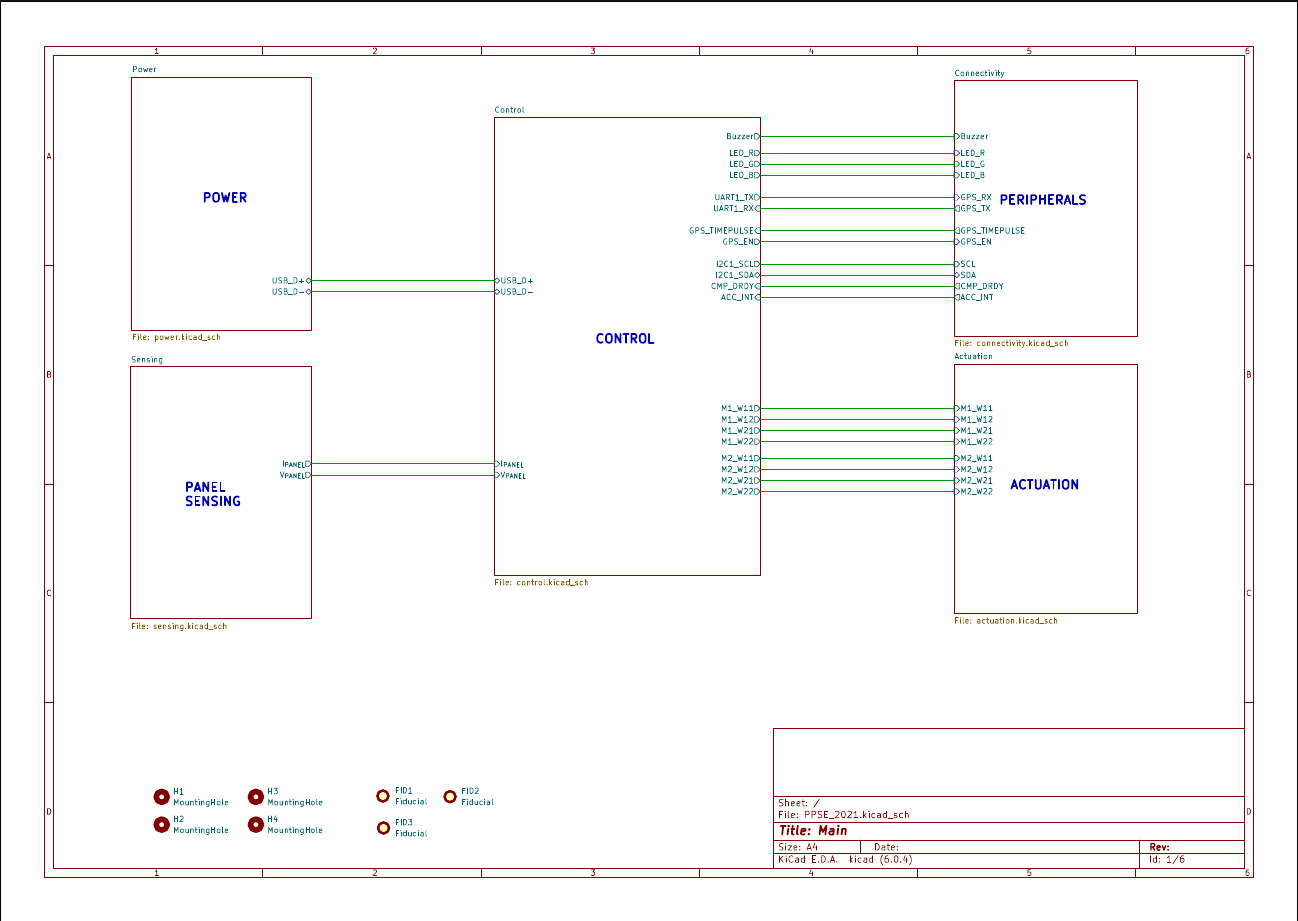
\includegraphics[width=6.5in,height=4.48in]{figures/image32.png}
\captionsetup{type=figure}
\captionof{figure}{Foglio "Main" SALMO}
\end{center}

\hypertarget{control}{%
\section{Control}\label{control}}

Il foglio ``\emph{Control}'' include i componenti adibiti al controllo
della scheda, quali:

\begin{itemize}
\item
  \begin{quote}
  microcontrollore \emph{RP2040};
  \end{quote}
\item
  \begin{quote}
  memoria flash SPI \emph{W25Q16JV};
  \end{quote}
\item
  \begin{quote}
  cristallo al quarzo a 12 \emph{MHz};
  \end{quote}
\item
  \begin{quote}
  pulsanti di reset, boot, home e tracking enable;
  \end{quote}
\item
  \begin{quote}
  connettori di debug ed espansione.
  \end{quote}
\end{itemize}

\begin{center}
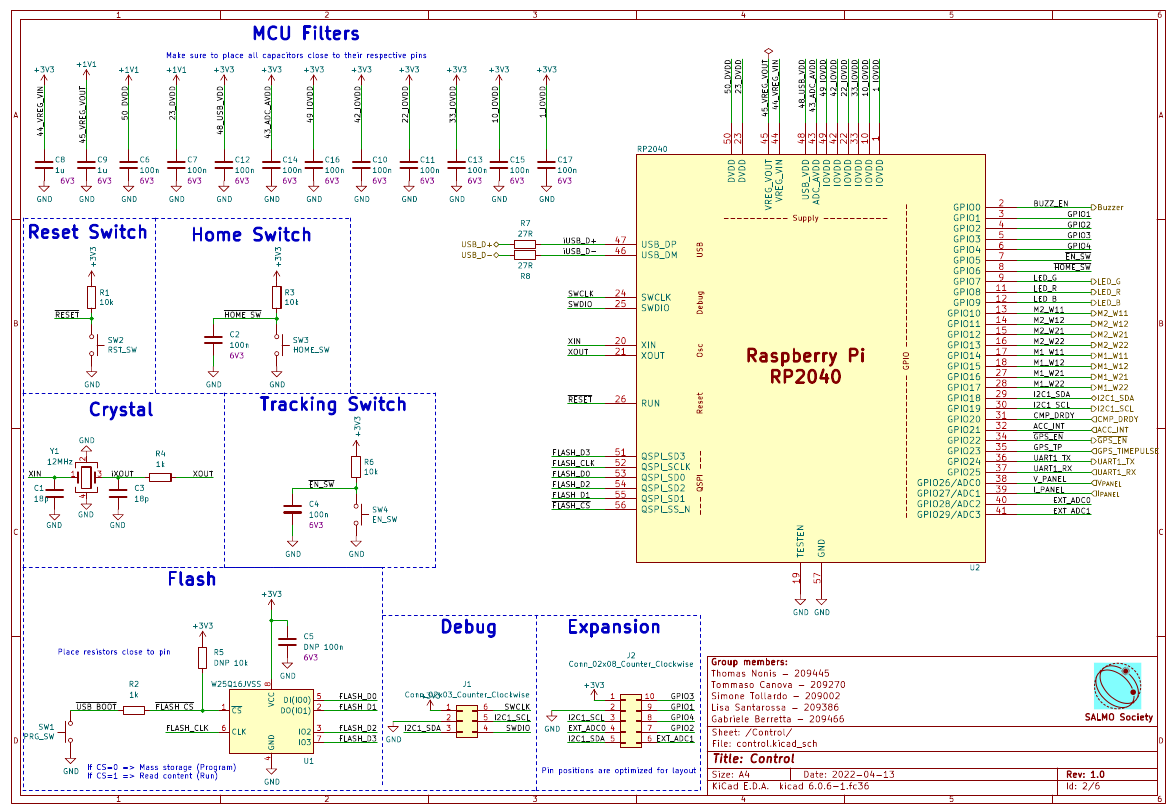
\includegraphics[width=6.5in,height=4.48611in]{figures/image40.png}
\captionsetup{type=figure}
\captionof{figure}{Foglio "Control" SALMO}
\end{center}

\hypertarget{microcontrollore-rp-2040}{%
\subsubsection{\texorpdfstring{\hfill\break
Microcontrollore: RP
2040}{ Microcontrollore: RP 2040}}\label{microcontrollore-rp-2040}}

La scheda si avvale dell'ormai celeberrimo \emph{MCU} di Raspberry Pi Ltd: \emph{RP2040}.

Caratteristiche principali:

\begin{itemize}
\item
  \begin{quote}
  133 \emph{MHz} dual core 32 bit ARM Cortex-M0+;
  \end{quote}
\item
  \begin{quote}
  264 \emph{KB} SRAM;
  \end{quote}
\item
  \begin{quote}
  Nessuna memoria flash interna;
  \end{quote}
\item
  \begin{quote}
  Controller bus \emph{QSPI}, che supporta fino a 16 MB di memoria flash
  esterna;
  \end{quote}
\item
  \begin{quote}
  Controllore \emph{DMA};
  \end{quote}
\item
  \begin{quote}
  Crossbar \emph{AHB} (Advanced High-performance Bus);
  \end{quote}
\item
  \begin{quote}
  Regolatore \emph{LDO} programmabile per generare la tensione del core
  integrato;
  \end{quote}
\item
  \begin{quote}
  2 \emph{PLL} su chip per generare clock USB e core;
  \end{quote}
\item
  \begin{quote}
  30 pin \emph{GPIO}, di cui 4 utilizzabili opzionalmente come ingressi
  analogici.
  \end{quote}
\end{itemize}

Periferiche:

\begin{itemize}
\item
  \begin{quote}
  2 \emph{UART};
  \end{quote}
\item
  \begin{quote}
  2 controller \emph{SPI};
  \end{quote}
\item
  \begin{quote}
  2 controller \emph{I²C};
  \end{quote}
\item
  \begin{quote}
  16 canali \emph{PWM};
  \end{quote}
\item
  \begin{quote}
  Controller USB 1.1 e \emph{PHY}, con supporto per host e dispositivo;
  \end{quote}
\item
  \begin{quote}
  8 macchine a stati di input-output (\emph{PIO}) programmate.
  \end{quote}
\end{itemize}

Il microcontrollore ha il compito di gestire le periferiche. In
particolare:

\begin{itemize}
\item
  \begin{quote}
  genera il segnale di rotazione dei motori quando previsto
  dall'algoritmo implementato (\emph{GPIO} da 10 a 17);
  \end{quote}
\item
  \begin{quote}
  comunica con il GPS tramite interfaccia UART (\emph{GPIO} 24 e 25);
  \end{quote}
\item
  \begin{quote}
  comunica con il magnetometro, con l'accelerometro e con il display
  OLED mediante interfaccia I2C (\emph{GPIO} 18 \emph{SDA}, \emph{GPIO}
  19 \emph{SCL});
  \end{quote}
\item
  \begin{quote}
  effettua le misure di corrente e di tensione del pannello (\emph{GPIO}
  26 e 27);
  \end{quote}
\item
  \begin{quote}
  gestisce il buzzer (\emph{GPIO} 0) ed un led \emph{RGB} (\emph{GPIO}
  7, 8, 9);
  \end{quote}
\item
  \begin{quote}
  comunica con la memoria \emph{flash} (pin da 51 a 56);
  \end{quote}
\item
  \begin{quote}
  gestisce l'interfaccia \emph{USB} (pin 46 e 47).
  \end{quote}
\end{itemize}

\begin{center}
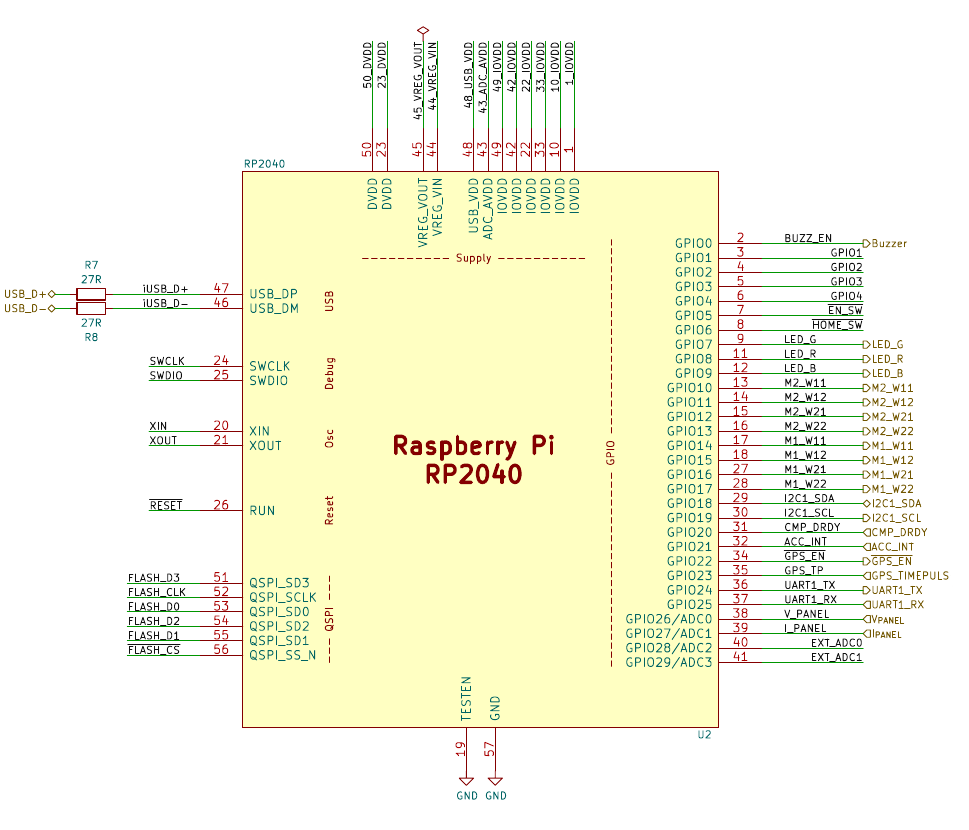
\includegraphics[width=6.5in,height=5.56944in]{figures/image54.png}
\captionsetup{type=figure}
\captionof{figure}{Schema pin microcontrollore RP2040\newline}
\end{center}

Per ridurre il rumore ad alta frequenza presente sulla linea di
alimentazione abbiamo previsto dei condensatori di filtro per
cortocircuitare a massa la componente alternata (andranno poi
posizionati il più vicino possibile ai pin del MCU).

\begin{center}
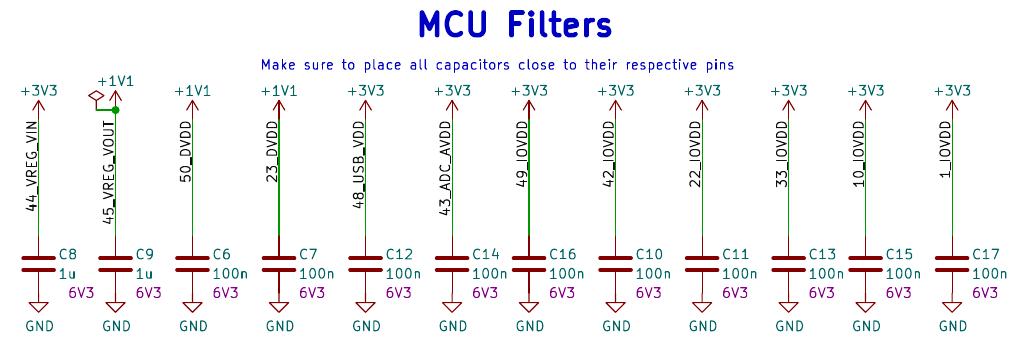
\includegraphics[width=6.33776in,height=2.22396in]{figures/image23.png}
\captionsetup{type=figure}
\captionof{figure}{Condensatori di bypass MCU}
\end{center}

\hypertarget{pulsanti}{%
\subsubsection{\texorpdfstring{\hfill\break
Pulsanti}{ Pulsanti}}\label{pulsanti}}

Per il progetto \emph{SALMO} abbiamo previsto quattro switch:

\begin{itemize}
\item
  \begin{quote}
  Un pulsante di reset (\emph{SW2}) per poter resettare il
  microcontrollore;
  \end{quote}
\item
  \begin{quote}
  Un pulsante per portare il microcontrollore in modalità
  \emph{bootloader (SW1)}, in modo tale da poter ``flashare'' il
  programma via USB.
  \end{quote}
\item
  \begin{quote}
  Un pulsante (\emph{SW3}), denominato "Home", che permette di portare
  il sistema di puntamento del pannello solare ad una posizione
  predefinita (0° Nord, 45° Elevazione);
  \end{quote}
\item
  \begin{quote}
  Un pulsante (\emph{SW4}), denominato ``Tracking Enable'', che permette
  di far partire il sistema di puntamento del pannello;
  \end{quote}
\end{itemize}

\begin{center}
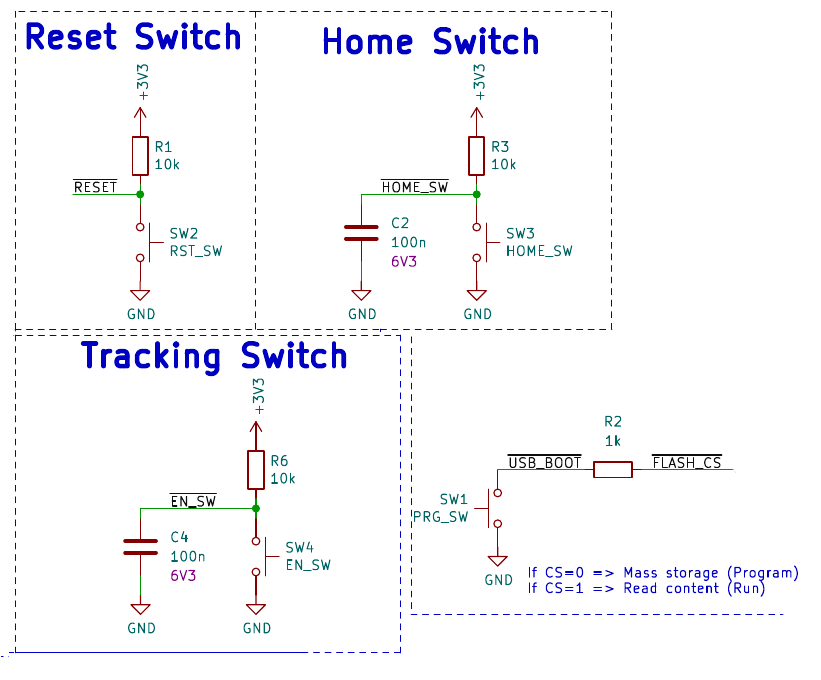
\includegraphics[scale=0.5]{figures/image16.png}
\captionsetup{type=figure}
\captionof{figure}{Pulsanti SALMO}
\end{center}

Per ogni pulsante abbiamo previsto un resistore di pull-up da 10kΩ, che
nel caso del pulsante di programmazione è contrassegnato come \emph{DNP}
(Do Not Place), poiché la memoria fornisce un \emph{pull-up} interno che
lo rende non necessario.

Per i pulsanti di \emph{reset} e programmazione non abbiamo previsto
alcun filtro di debouncing come consigliato dai relativi datasheet,
mentre per i restanti abbiamo aggiunto un condensatore da \emph{100nF}
per introdurre una costante di tempo di \emph{1ms}.

La resistenza R2 in serie al pulsante di programmazione è stata inserita
seguendo i consigli del manuale di sviluppo hardware del RP2040
(probabilmente il pin $\overline{\rm {CS}}$ della flash non ha una
resistenza di limitazione interna).

I pulsanti scelti sono dei generici \emph{tactile switch} da 6mm a
tecnologia TH .

\hypertarget{quarzo}{%
\subsubsection{Quarzo}\label{quarzo}}

Per generare il segnale di clock del microcontrollore abbiamo
selezionato un quarzo da 12 \emph{MHz}. In particolare abbiamo
utilizzato un quarzo a 4 pin con package \emph{3225}, essendo questo uno
dei constraint imposti dal professore ad inizio progetto. Per il
dimensionamento del resistore in serie e dei condensatori abbiamo
seguito le linee guida del manuale di sviluppo hardware del RP2040.

\(C_{1} = C_{2} = 2 \cdot (C_{L} - C_{\text{Parassita}})\)
, dove \(C_{L}\) è la capacità di load ottimale del quarzo.

Ipotizzando quindi una capacità parassita pari a 5pF ed una capacità di
load di 14pF otteniamo \(C_{1} = C_{2} =18pF\).

\begin{center}
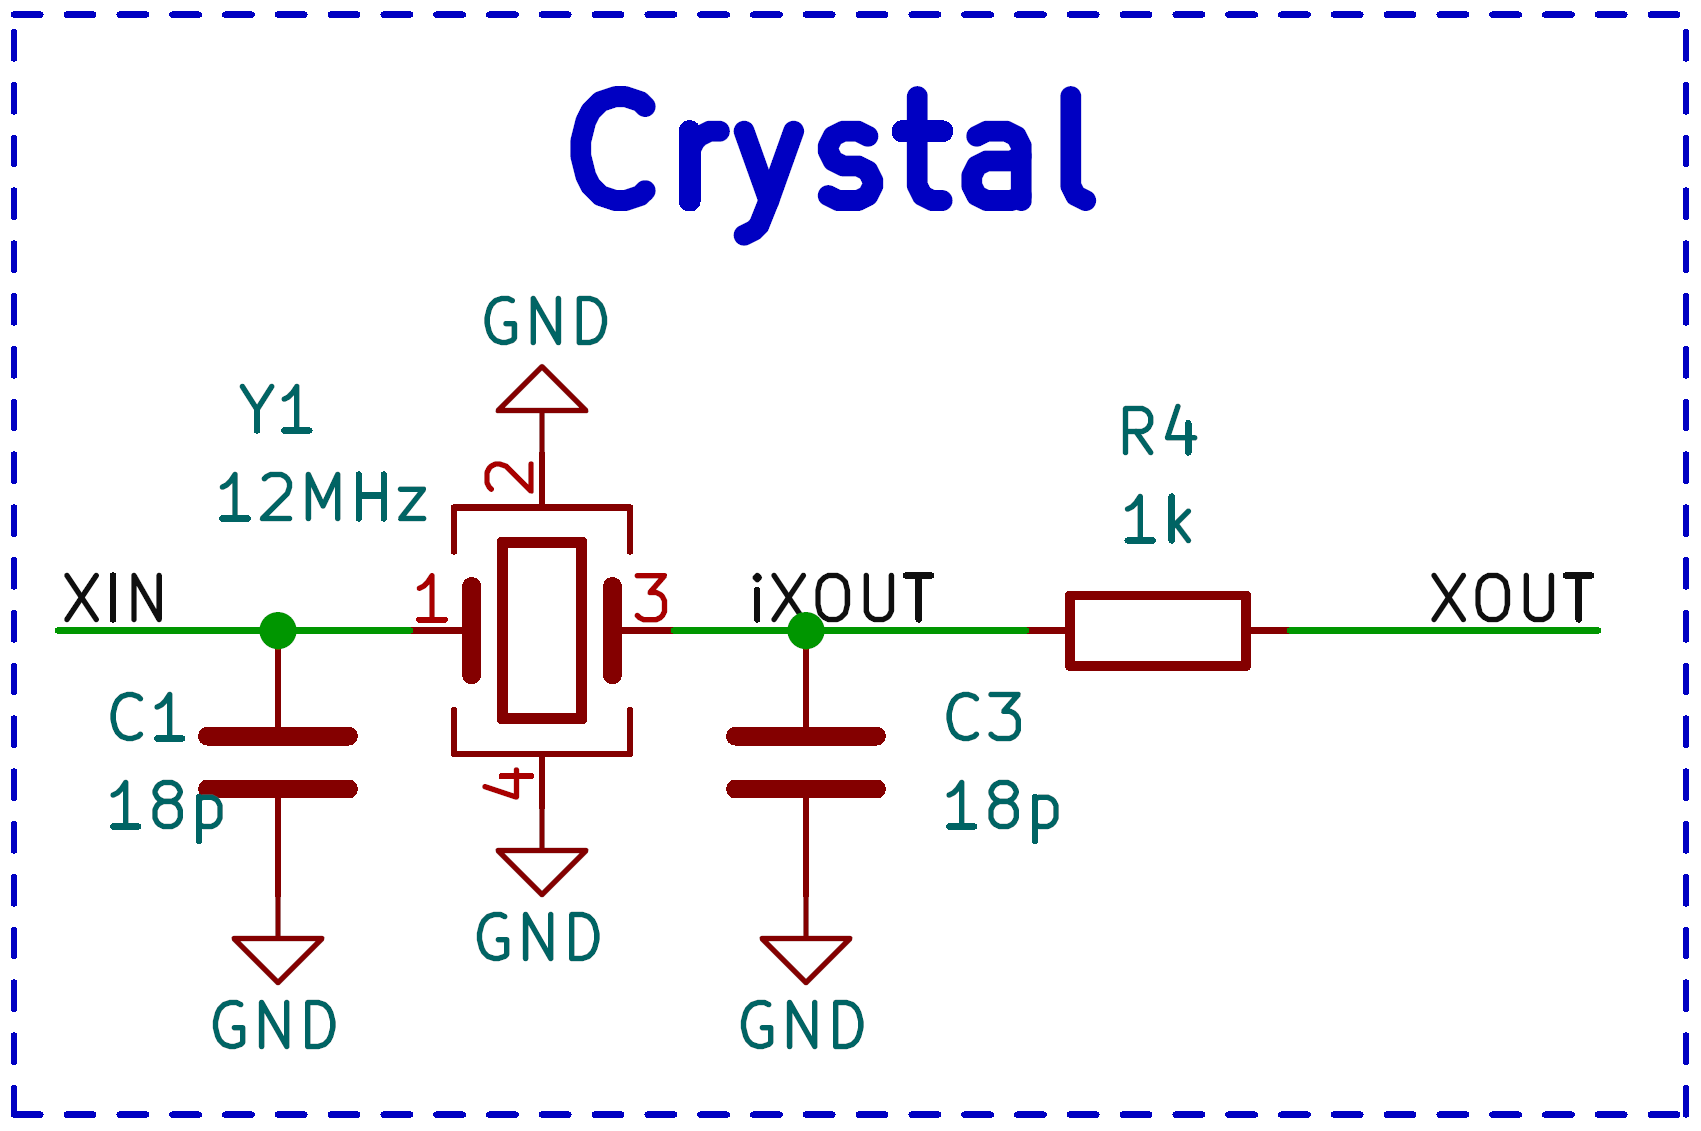
\includegraphics[scale=0.8]{figures/image76.png}
\captionsetup{type=figure}
\captionof{figure}{Circuito del cristallo di quarzo di SALMO\newline}
\end{center}

La capacità di carico è particolarmente importante perché, essendo la
capacità totale vista dai due pin del cristallo XIN e XOUT, può portare
il cristallo ad oscillare in un punto specifico tra la sua frequenza
minima e massima. Cambiando la capacità del carico si otterrà quindi una
diversa frequenza di oscillazione. Ecco perché il produttore di
cristalli fornisce la frequenza del cristallo a una capacità di carico
specifica, che in questo caso è di 14pF.

\begin{center}
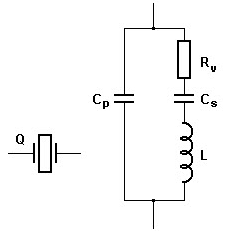
\includegraphics[width=2.38542in,height=2.45833in]{figures/image28.png}
\captionsetup{type=figure}
\captionof{figure}{Modello RLC di un cristallo al quarzo in risonanza parallelo}
\end{center}

\hypertarget{memoria-flash}{%
\subsubsection{\texorpdfstring{\hfill\break
Memoria flash}{ Memoria flash}}\label{memoria-flash}}

Nella memoria flash viene salvato il firmware compilato in formato
\emph{.uf2}, il quale all'accensione verrà eseguito dal bootloader. La
memoria flash utilizzata è la \emph{W25Q16JV}, e viene interfacciata
mediante protocollo QSPI (Quad-SPI). Questo tipo di comunicazione è
particolarmente diffuso nel ramo delle comunicazioni con memorie flash,
come nel caso presente sulla scheda. Rispetto allo standard SPI, sono
presenti 4 linee di dato bidirezionali, rispettivamente \emph{I0, I1,
I2, I3} (che vanno dunque a sostituire \emph{MISO} e \emph{MOSI}), che
permettono un trasferimento dati più veloci dalle 4 alle 6 volte
rispetto normale SPI (secondo il datasheet).

\begin{center}
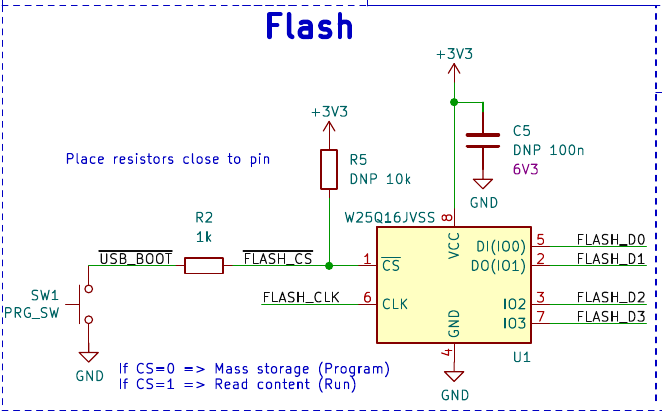
\includegraphics[width=6.5in,height=4.05556in]{figures/image49.png}
\captionsetup{type=figure}
\captionof{figure}{Circuito flash SALMO}
\end{center}

Il pin $\overline{\rm {CS}}$ permette di abilitare o
disabilitare la comunicazione \emph{QSPI}, quando $\overline{\rm {CS}}$=1 i pin di
comunicazione rimangono ad alta impedenza, mentre quando $\overline{\rm {CS}}$=0 è
possibile interfacciarsi con la memoria per memorizzare il programma. È
inoltre presente un condensatore da 100nF per filtrare rumore ad alta
frequenza in alimentazione.

\hypertarget{debug-ed-espansione}{%
\subsubsection{\texorpdfstring{\hfill\break
Debug ed espansione}{ Debug ed espansione}}\label{debug-ed-espansione}}

\begin{center}
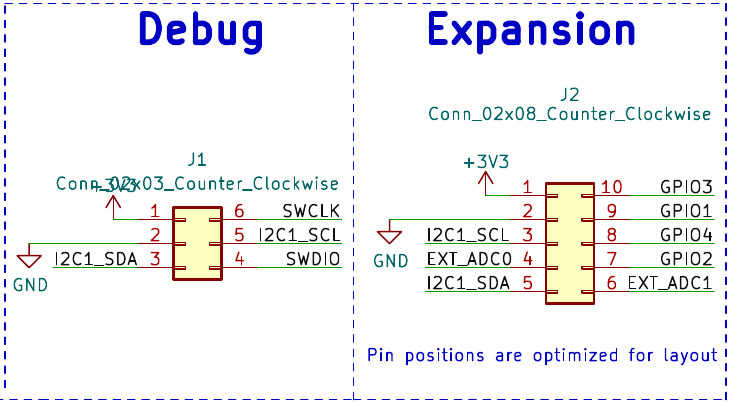
\includegraphics[scale=0.8]{figures/image90.png}
\captionsetup{type=figure}
\captionof{figure}{Connettori Debug ed Expansion SALMO\newline}
\end{center}

Per permettere al microcontrollore di comunicare con eventuali unità
esterne, sulla scheda abbiamo inserito un connettore a 10 pin con le
linee \emph{I2C}, i due canali non utilizzati del convertitore analogico
digitale ed i rimanenti \emph{GPIO} non utilizzati.\\
Abbiamo previsto anche un connettore per il debug con interfaccia SWD
(\emph{Serial Wire Debug}), alimentazione per il microcontrollore e bus
\emph{I2C}. Per il debug è necessario utilizzare un altro \emph{RP2040},
potrebbe essere particolarmente conveniente utilizzare un Pi Pico come
debugger, viste le due dimensioni. Basta collegare le linee di SWData e
SWClock tra loro e la relativa alimentazione necessaria al debugger,
dopodichè si può flashare quest'ultimo con \emph{picoprobe.uf2}
(programma situato nella cartella degli esempi offerti per RP2040,
vedesi capitolo
\protect\hyperlink{_w8kvxnysumpc}{\underline{Firmware}}), per poi
interfacciarsi via usb utilizzando GDB ed OpenOCD.

\begin{center}
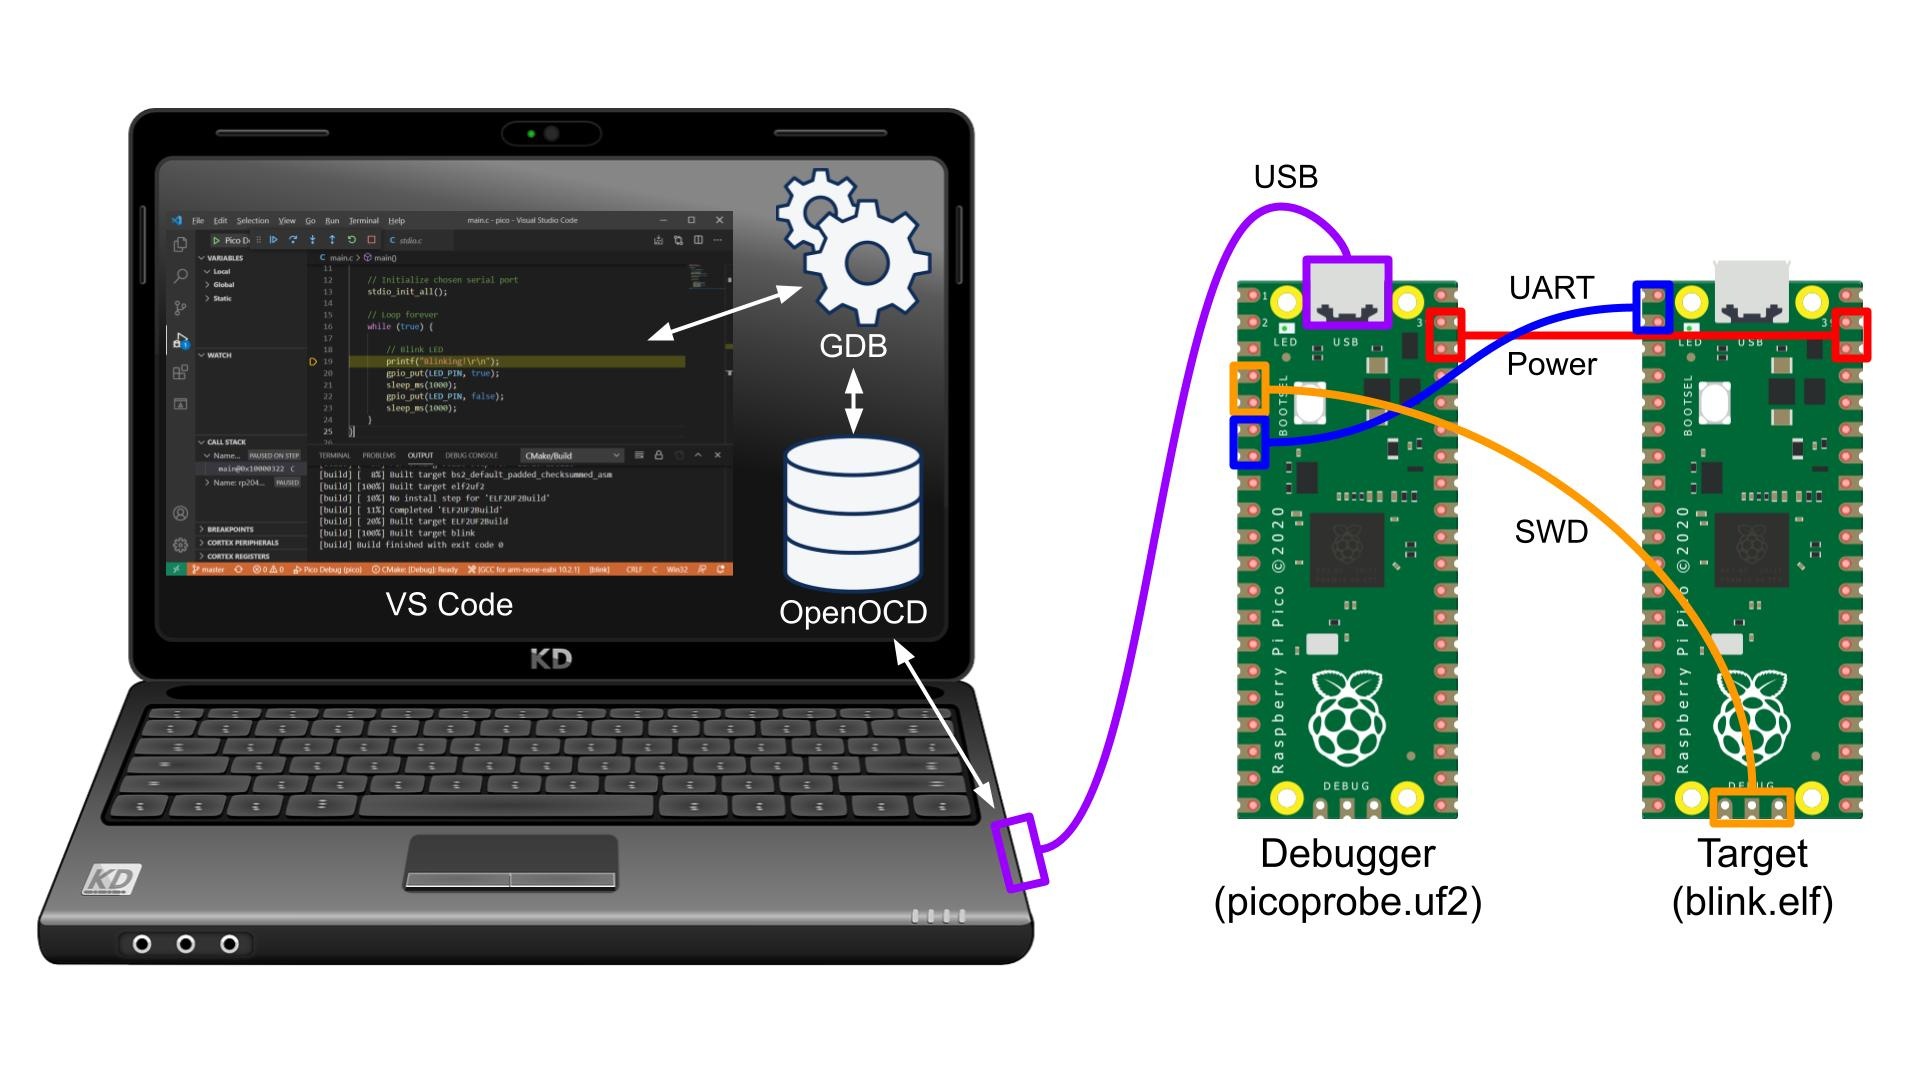
\includegraphics[width=6.5in,height=3.65278in]{figures/image18.png}
\captionsetup{type=figure}
\captionof{figure}{Immagine illustrativa del debug di un Pi Pico mediante un altro Pi Pico}
\end{center}

\hypertarget{power}{%
\section{Power}\label{power}}

\begin{center}
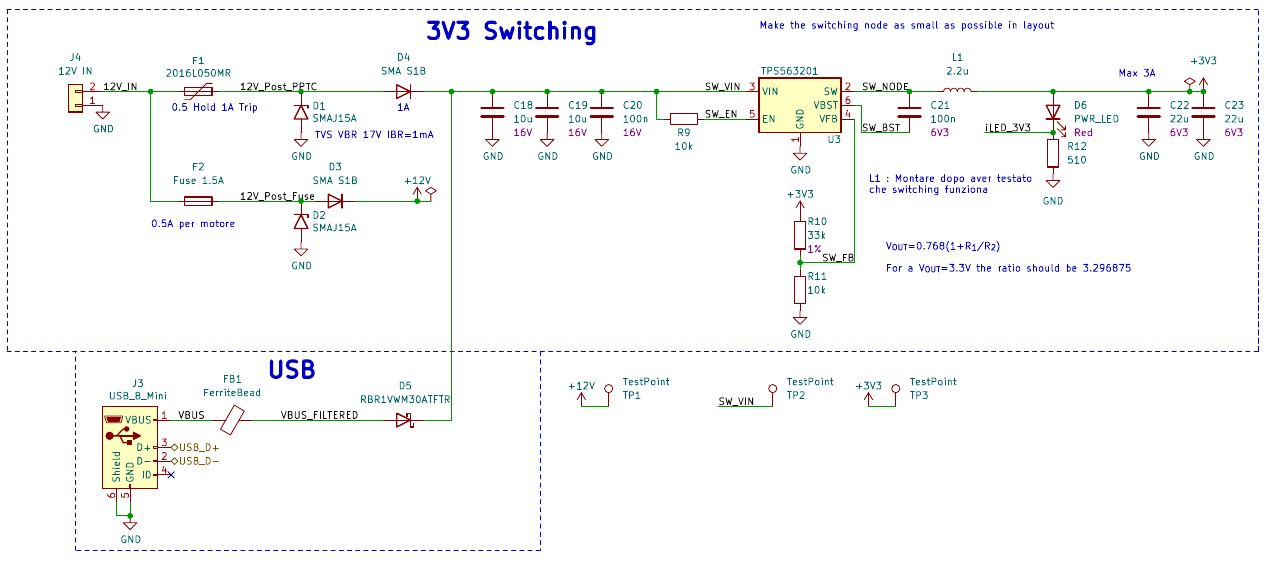
\includegraphics[width=6.5in,height=3.65278in]{figures/image65.png}
\captionsetup{type=figure}
\captionof{figure}{Foglio "Power" SALMO\newline}
\end{center}

L'alimentazione principale della scheda (+12V) proviene dal connettore
J4 e verrà successivamente ``divisa'' in due rami: regolatore di
tensione e alimentazione dei motori.

\begin{center}
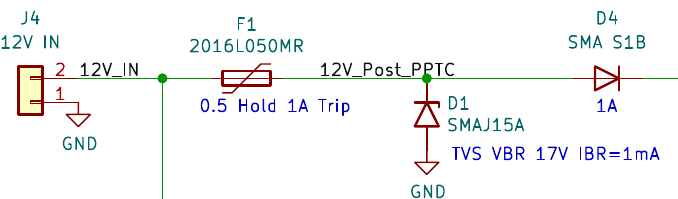
\includegraphics[scale=0.8]{figures/image80.png}
\captionsetup{type=figure}
\captionof{figure}{Ramo regolatore di tensione\newline}
\end{center}

\begin{center}
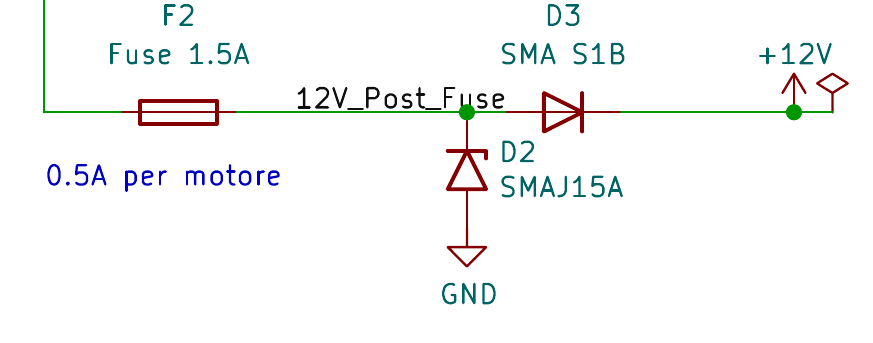
\includegraphics[scale=0.6]{figures/image64.png}
\captionsetup{type=figure}
\captionof{figure}{Ramo alimentazione motori\newline}
\end{center}

La scheda può essere alimentata anche tramite un connettore \emph{USB}
di tipo B-mini (il pin \emph{ID} è stato lasciato flottante non dovendo
utilizzare la funzione \emph{USB OTG}, fissando il dispositivo come
device), ovviamente non potendo alimentare motori e led \emph{RGB}.\\
Per evitare i rumori ad alta frequenza la tensione di bus viene filtrata
tramite una \emph{ferrite bead}, la quale sfrutta le medesime proprietà
dell'induttore, esercitando una resistenza 120 Ω a 100 MHz.

È necessaria inoltre la presenza del diodo schottky \emph{D5} per
evitare che i 12V possano propagarsi fino alla rail dei 5V dell'USB.

\begin{center}
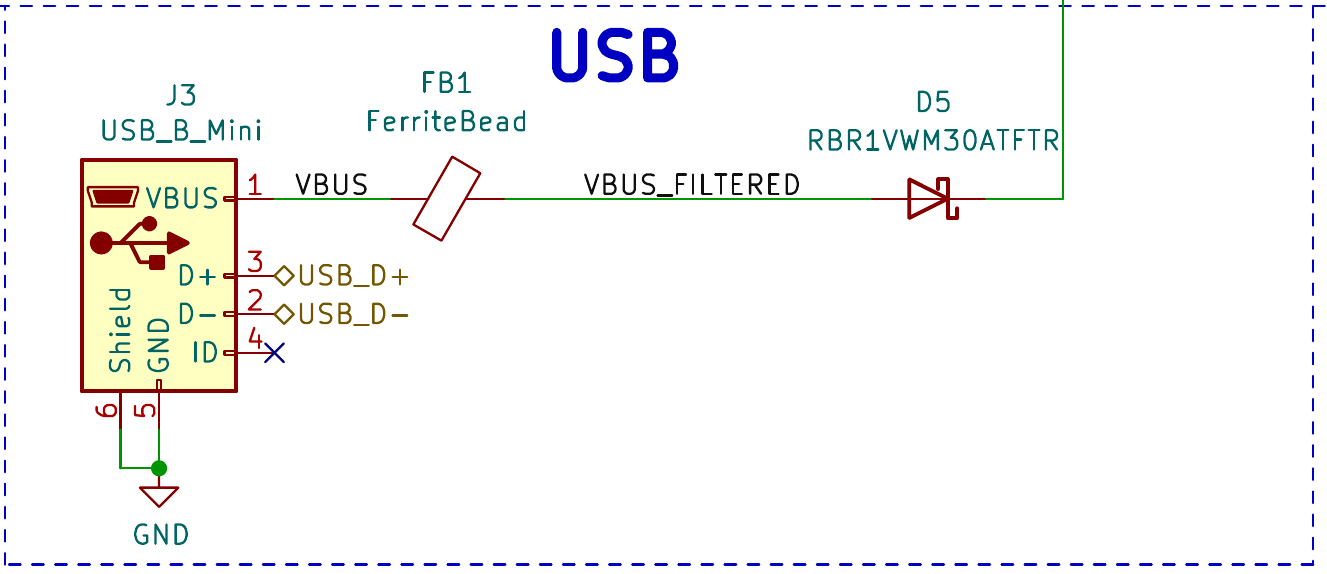
\includegraphics[width=6.5in,height=2.80556in]{figures/image60.png}
\captionsetup{type=figure}
\captionof{figure}{Alimentazione via USB\newline}
\end{center}

I diodi \emph{D4} e \emph{D5} sono imperativi e svolgono la funzione di
\emph{OR logico} per garantire in ogni caso l'alimentazione al
regolatore switching.

Il fusibile \emph{F2} serve per proteggere i driver dei motori ed i
motori stessi dalle sovracorrenti, mentre a protezione del
microcontrollore e delle periferiche è stato previsto il fusibile
resettabile \emph{F1}, un \emph{PPTC} (polymeric positive temperature
coefficient). Quest'ultimo è in grado di aumentare la sua resistenza
all'aumentare della temperatura, riducendo così il passaggio di corrente
nel ramo.\\
La corrente massima assorbita da ciascun motore è di circa 0.5 A, perciò
abbiamo scelto un fusibile da 1.5 A (lasciando qualche centinaio di mA
per il led \emph{RGB} e qualche altro per avere una minima
tolleranza).\\
Il diodo \emph{SMAJ15A} è invece un diodo TVS, cioè un dispositivo
\emph{p-n} studiato per assorbire correnti elevate di eventi transitori
elettrici.

Il regolatore di tensione utilizzato è un \emph{TPS563201}, con tensione
in ingresso minima di 4.5V e massima di 17V. Per poter avere in output
una tensione di 3.3V, il pin VFB del regolatore deve essere connesso tra
due resistenze di rapporto \(\frac{R10}{R11} = \ 3.3\) considerando che
la formula per dimensionare Vout, ottenuta dal datasheet, è
\(Vout = 0.768(1 + \frac{R10}{R11})\).\\
Al fine di segnalare la presenza dei 3.3V, abbiamo previsto un led rosso
con resistenza in serie da 510 Ω.

\begin{center}
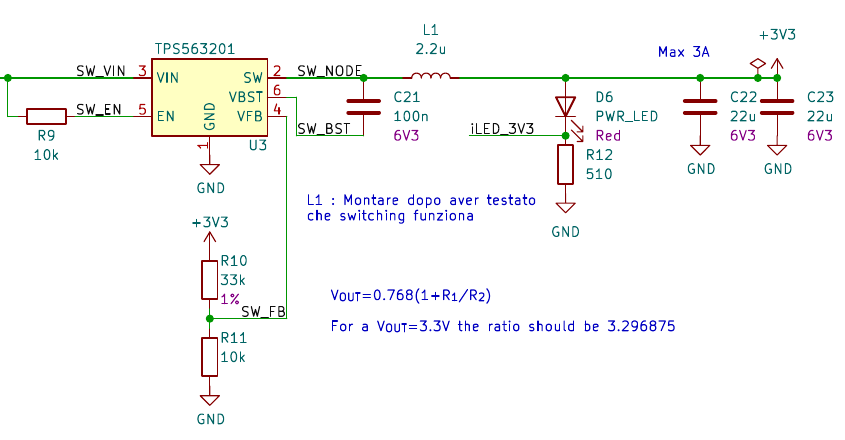
\includegraphics[scale=0.7]{figures/image57.png}
\captionsetup{type=figure}
\captionof{figure}{Circuito regolatore di tensione buck}
\end{center}

All'ingresso del regolatore di tensione abbiamo posto tre condensatori
(due da 10u e uno da 100n) con lo scopo di ridurre il ripple in uscita
dal regolatore switching. Si inseriscono 3 condensatori poiché, essendo
componenti reali e presentando di conseguenza una resistenza ed una
induttanza parassita, la loro combinazione darà luogo ad un condensatore
con caratteristiche migliori rispetto ad un condensatore di capacità
pari alla loro somma.

\begin{center}
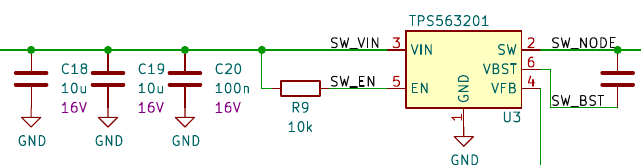
\includegraphics[scale=0.8]{figures/image71.png}
\captionsetup{type=figure}
\captionof{figure}{Condensatori in ingresso al regolatore di tensione\newline}
\end{center}

\begin{center}
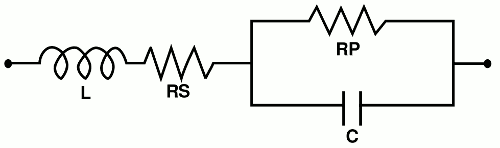
\includegraphics[scale=0.8]{figures/image37.png}
\captionsetup{type=figure}
\captionof{figure}{Modello RLC di un condensatore reale\newline}
\end{center}

Abbiamo infine previsto dei test point per il controllo delle varie
tensioni sul pannello.

\begin{center}
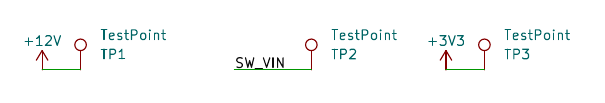
\includegraphics[scale=1]{figures/image78.png}
\captionsetup{type=figure}
\captionof{figure}{Testpoint per la misura delle tensioni di alimentazione}
\end{center}

\hypertarget{peripherals}{%
\section{Peripherals}\label{peripherals}}

\begin{center}
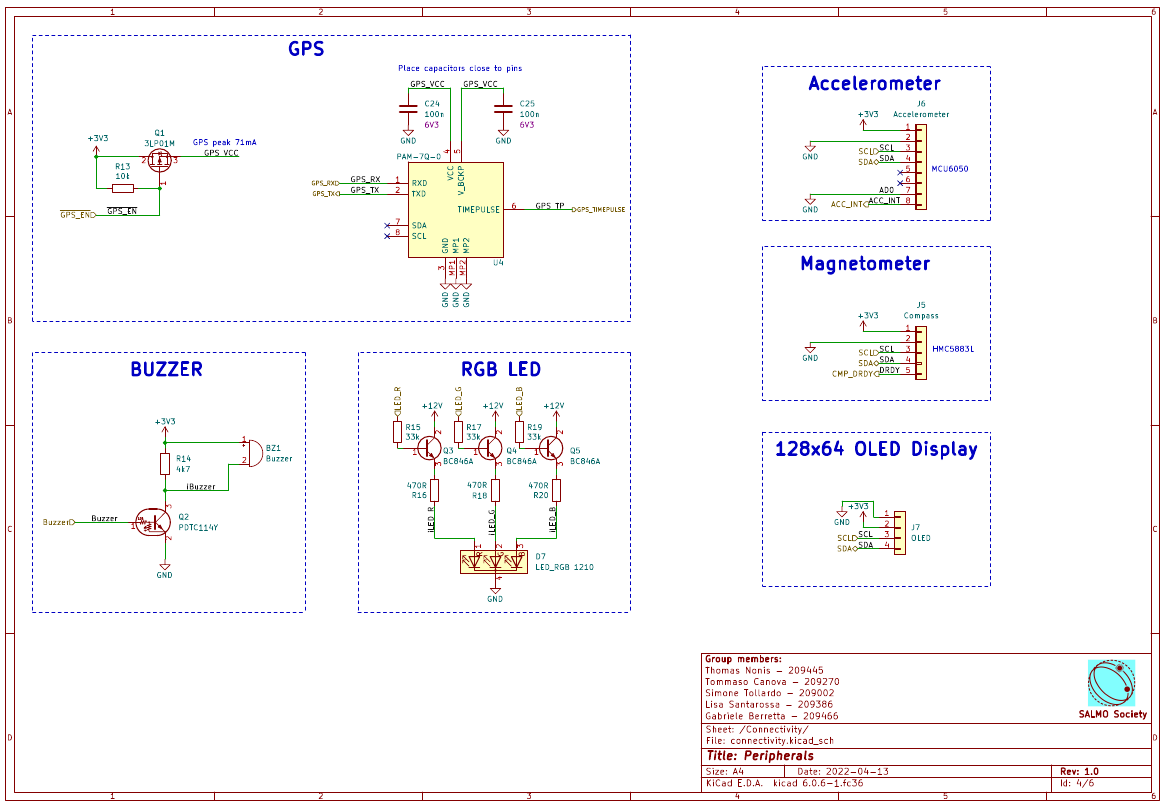
\includegraphics[width=6.5in,height=4.48611in]{figures/image15.png}
\captionsetup{type=figure}
\captionof{figure}{Foglio "Peripherals" SALMO}
\end{center}

\hypertarget{gps}{%
\subsubsection{\texorpdfstring{\hfill\break
\hfill\break
GPS }{  GPS }}\label{gps}}

Il dispositivo \emph{GPS} utilizzato è il \emph{U-BLOX PAM7Q}. Questo
componente serve per poter ottenere dai satelliti e la coordinate
geografiche del dispositivo \emph{SALMO}, in modo tale che il
microcontrollore possa calcolare la posizione del Sole rispetto al
pannello attraverso l'algoritmo di tracciamento e successivamente
stabilire il movimento dei motori.\\
Il dispositivo utilizza il protocollo standard \emph{NMEA} (ma può
essere configurato anche per utilizzare il protocollo proprietario
\emph{U-BLOX}) per comunicare attraverso la linea seriale.

\begin{center}
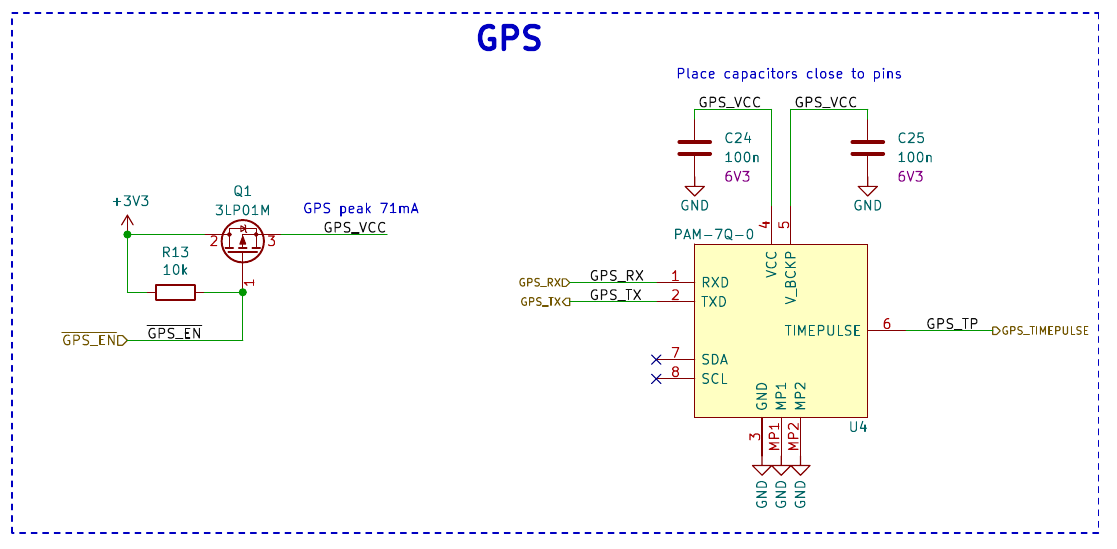
\includegraphics[width=6.5in,height=3.19444in]{figures/image26.png}
\captionsetup{type=figure}
\captionof{figure}{Circuito del GPS PAM7Q\newline}
\end{center}

Il dispositivo è alimentato a \emph{3V3} tramite i pin 4 e 5, si noti
che \emph{V\_BCKP} e \emph{VCC} sono entrambe connesse alla stessa
alimentazione, in quanto non è stata prevista una batteria tampone. Sono
presenti nuovamente i condensatori da 100nF tra \emph{GPS\_VCC} e ground
servono a bypassare il rumore ad alta frequenza verso massa.

L'alimentazione è interrotta da un transistor \emph{PMOS} (\emph{Q1}) e
viene abilitata solo quando il transistor viene polarizzato
correttamente, ovvero quando \textasciitilde(\emph{GPS\_EN}) si trova a
livello logico basso. La resistenza da 10kΩ tra gate e source del pmos
serve a mantenere il transistor in cut off quando il pin
\textasciitilde(\emph{GPS\_EN}) non è pilotato (floating).\\
I pin 1 e 2, cioè \emph{RXD} e \emph{TXD}, sono rispettivamente i pin di
ricezione e trasmissione per la comunicazione \emph{UART} (rispetto al
\emph{GPS}).\\
Il pin 6 è dedicato al time pulse, ovvero a generare un segnale
elettrico a 1 \emph{PPS} (pulse per second). Questa uscita può essere
utilizzata, ad esempio, per riattivare l'MCU da una modalità di
sospensione una volta al secondo per comunicare con esso. Il \emph{GPS}
\emph{PAM7Q} presenta anche un interfaccia seriale \emph{I2C} ma, dato
che per il progetto \emph{SALMO} abbiamo scelto un interfacciamento via
\emph{UART,} i pin 7 e 8 (\emph{SDA} e \emph{SCL}) sono stati lasciati
flottanti.\\
I mounting point \emph{MP1} e \emph{MP2} sono collegati a massa come
indicato da datasheet.

\begin{center}
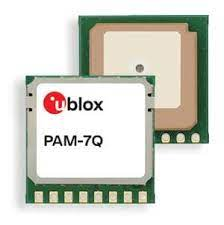
\includegraphics[scale=0.8]{figures/image30.jpg}
\captionsetup{type=figure}
\captionof{figure}{GPS U-Blox PAM7Q}
\end{center}

\hypertarget{magnetometro-ed-accelerometro}{%
\subsubsection{\texorpdfstring{\hfill\break
Magnetometro ed Accelerometro\\
}{ Magnetometro ed Accelerometro }}\label{magnetometro-ed-accelerometro}}

Al fine di poter gestire la posizione del pannello mediante controllo ad
anello chiuso abbiamo deciso di sfruttare due sensori: un magnetometro a
3 assi a 12 bit \emph{Honeywell} \emph{HMC5883L} ed un
accelerometro+giroscopio entrambi a 3 assi a 16 bit \emph{TDK}
\emph{MPU6050}, tutti e 2 con interfaccia \emph{I2C} a 400KHz massimi.\\
Questi, saranno posizionati \textbf{direttamente sul pannello} e
provvederanno a restituire all'algoritmo la posizione del pannello
rispetto ai due assi di movimento (Azimuth ed Elevazione).

Tuttavia, non avendo avuto a disposizione l'accelerometro durante la
fase di assemblaggio, in questa release non è fisicamente presente.

\begin{center}
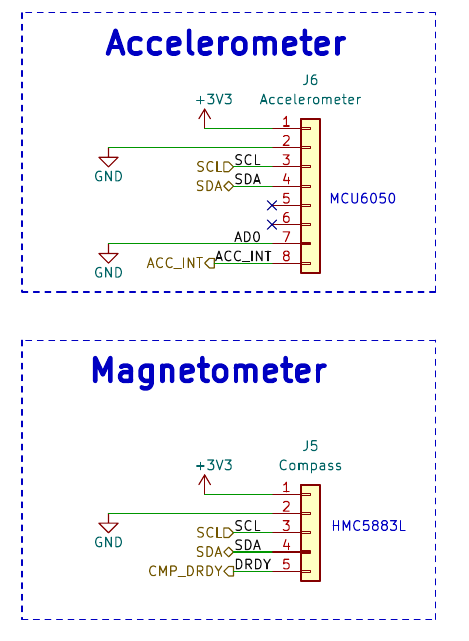
\includegraphics[scale=0.6]{figures/image31.png}
\captionsetup{type=figure}
\captionof{figure}{Connettori Accelerometro e Magnetometro}
\end{center}

\hypertarget{connettore-display-oled}{%
\subsubsection{\texorpdfstring{Connettore display OLED\\
}{Connettore display OLED }}\label{connettore-display-oled}}

Abbiamo previsto un connettore per un display \emph{OLED 128 x 64} con
controller integrato \emph{SSD1306} al fine di presentare all'utente una
immediata visualizzazione dei dati della scheda e del pannello solare.\\
Tuttavia, non avendo avuto a disposizione il componente durante la fase
di assemblaggio, in questa release non è fisicamente presente.

\begin{center}
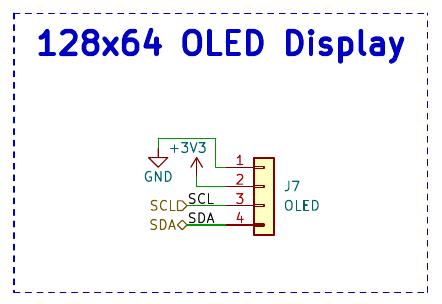
\includegraphics[scale=0.7]{figures/image58.png}
\captionsetup{type=figure}
\captionof{figure}{Connettore display OLED 128x64}
\end{center}

\hypertarget{led-rgb}{%
\subsubsection{\texorpdfstring{\hfill\break
\hfill\break
LED RGB}{  LED RGB}}\label{led-rgb}}

Per quanto riguarda il circuito del led \emph{RGB 1210} abbiamo commesso
un errore in fase di progettazione: considerandone la posizione, tra
collettore ed emettitore del transistor cadranno circa
12-(3.3-0.7)=9.4V!\\
Conseguentemente ai capi dei diodi led cadrà una tensione molto bassa,
probabilmente nemmeno sufficiente per portarli in conduzione.\\
Purtroppo il problema non è sistemabile, se non modificando il circuito
ed il layout della PCB.

Considerando che il componente è del tutto ausiliario abbiamo potuto
testare comunque la scheda senza alcun problema.

\begin{center}
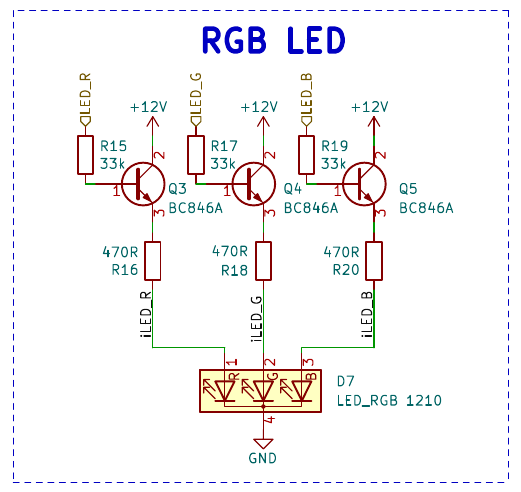
\includegraphics[width=3.68946in,height=3.49479in]{figures/image17.png}
\captionsetup{type=figure}
\captionof{figure}{Circuito led RGB 1210}
\end{center}

\hypertarget{buzzer}{%
\subsubsection{\texorpdfstring{\hfill\break
\hfill\break
Buzzer}{  Buzzer}}\label{buzzer}}

Abbiamo previsto un buzzer passivo di tipo elettromagnetico per poter
segnalare eventuali stati all'utente e/o errori. Per amplificare il
segnale proveniente dall'RP2040 abbiamo utilizzato un transistor NPN con
rete di polarizzazione integrata ed un resistore in parallelo al
cicalino per poter scaricare la tensione imposta dall'induttanza del
buzzer, che altrimenti danneggerebbe il transistor.

\begin{center}
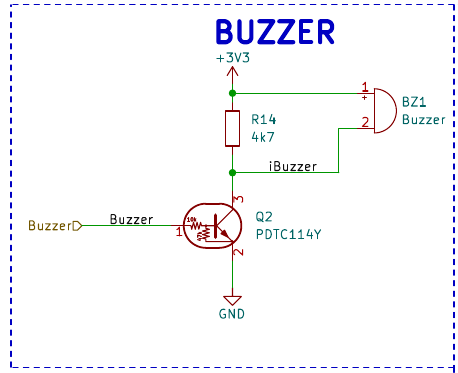
\includegraphics[width=3.08958in,height=2.51619in]{figures/image38.png}
\captionsetup{type=figure}
\captionof{figure}{Circuito buzzer}
\end{center}

\hypertarget{panel-sensing}{%
\section{\texorpdfstring{Panel sensing}{ Panel sensing}}\label{panel-sensing}}

\begin{center}
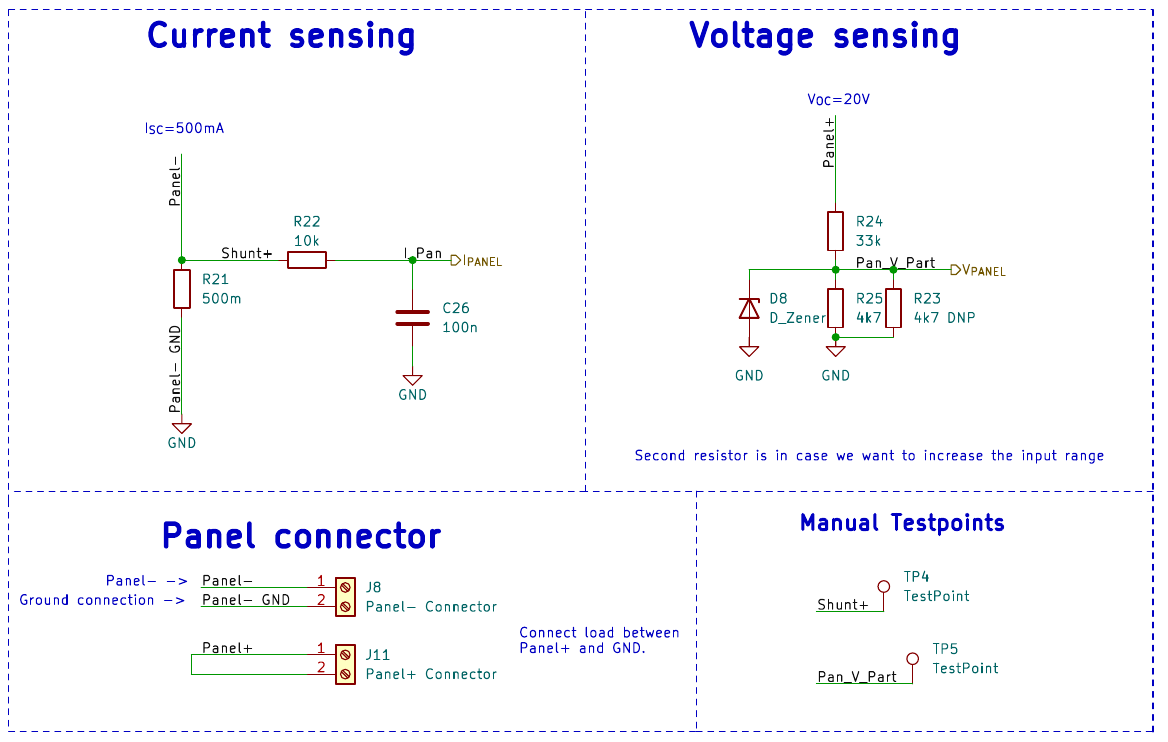
\includegraphics[width=6.5in,height=4.125in]{figures/image24.png}
\captionsetup{type=figure}
\captionof{figure}{Foglio "Panel Sensing" SALMO\newline}
\end{center}

Il panel sensing è stato progettato per la misura dei parametri di
tensione e di corrente del pannello solare. La misura di corrente del
pannello tiene conto di una corrente di cortocircuito (\emph{Isc}) pari
a \emph{500 mA}. Per effettuare la misura è stata posta una resistenza
di shunt pari a 500 mΩ per ottenere una misura di tipo \emph{low-side},
ottenendo così una caduta di tensione ai suoi capi massima di 0.25V che
può essere letta senza problemi dall'ADC dell'RP2040 (GPIO27, canale 2
dell'ADC).\\
Nella scelta della resistenza di shunt, condizionata dal fatto che non
volevamo complicare inutilmente il circuito con degli amplificatori
operazionali, è stato dato maggior peso alla potenza dissipata che allo
sfruttare in maniera ottimale il range dell'ADC.\\
La tensione misurata dall'ADC andrà infatti da 0V (Ipanel=0 A) a 0.25 V
(Ipanel=Isc=500 mA) e la potenza dissipata massima sarà quindi
\(R*I^{2}\  = 0.5*0.5^{2} = 0.125\ W\).\\
Avendo un \emph{ADC} a 12 bit, è possibile ottenere una sensibilità di
\(\frac{(Vref - Vss)}{2^{\text{bit}}} = \frac{3.3}{2^{12}} = 805.66\ uV/bit\)
, corrispondente a
\(\frac{(Vref - Vss)}{2^{\text{bit}}*0.5} = \frac{3.3}{2^{11}} = 1.6\ mA/bit\).
Data la Vmax di segnale pari a 0.25 V è possibile sfruttare solamente il
7.6\% dell'intero range disponibile
(\(\frac{\text{Vref}}{\text{Vmax}} = \frac{3.3}{0.25} = 7.26\%\))

\begin{center}
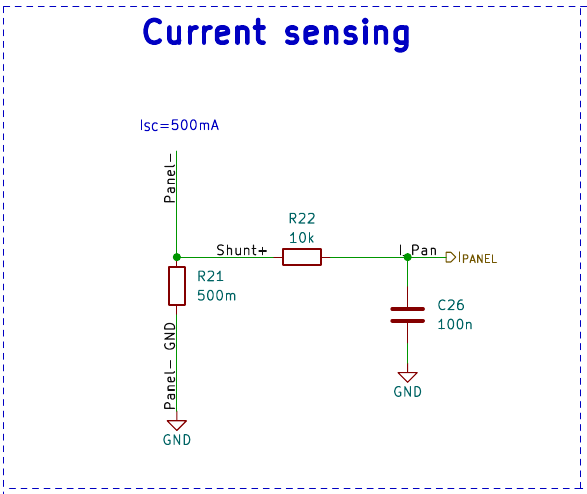
\includegraphics[width=4.19954in,height=3.53646in]{figures/image19.png}
\captionsetup{type=figure}
\captionof{figure}{Circuito Current Sensing SALMO\newline}
\end{center}

Per la misura di tensione del pannello, non volendo nuovamente
utilizzare amplificatori operazionali o integrati specifici, abbiamo
scelto di utilizzare il metodo del partitore di tensione, posizionando
due resistenze da 33k e 47k per avere un rapporto di partizione di circa
\(\frac{4,7}{4,7 + 33} \simeq \ 0.125\). Assumendo di avere un pannello
con tensione di open circuit \emph{Voc} di 20V, i valori in ingresso al
GPIO 26 (canale numero 1 dell'ADC) andranno da 0V a 2.5V (la tensione
massima è comunque fissata dal diodo zener di protezione posto in
parallelo).
\({V_{\text{PANE}{L - MAX}_{\text{ADC}}} = V}_{panel +}*(\frac{R_{25}}{R_{25} + R_{24}}) = 20*0.125\  = 2.5\ V\ \)

Nel caso in cui il pannello avesse tensione di open circuit più alta o
volessimo usare più pannelli in serie tra di loro è possibile montare la
resistenza ausiliaria R23, che permette di avere un rapporto di
partizione di 0.067.

\({V_{\text{PANE}{L - MAX}_{\text{ADC}}} = V}_{panel +}*(\frac{R_{25}}{R_{25} + R_{24}}) = 20*0.067\  = 1.34\ V\)

\begin{center}
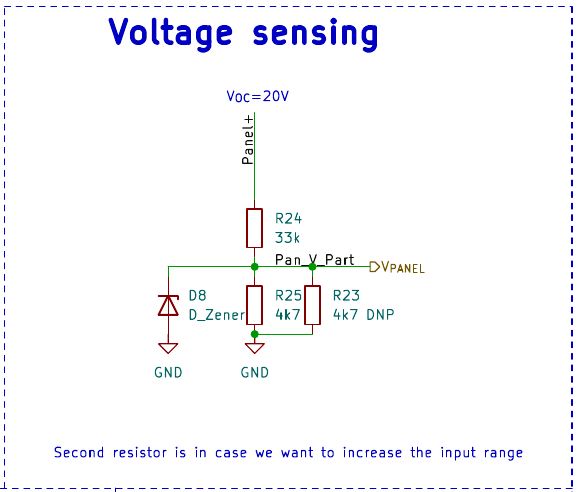
\includegraphics[scale=0.7]{figures/image62.png}
\captionsetup{type=figure}
\captionof{figure}{Circuito Voltage Sensing SALMO\newline}
\end{center}

In questo foglio abbiamo inoltre deciso di posizionare i connettori per
il collegamento del pannello e del relativo carico/utilizzatore.

\begin{center}
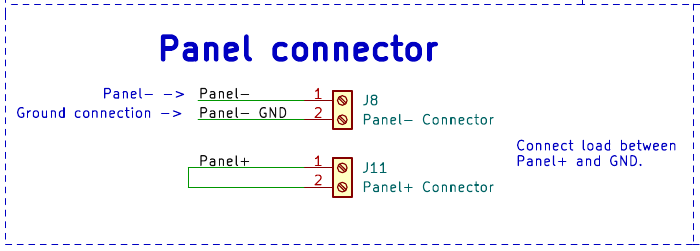
\includegraphics[scale=0.8]{figures/image48.png}
\captionsetup{type=figure}
\captionof{figure}{Connettori per carico e pannello SALMO\newline}
\end{center}

Abbiamo infine inserito dei test point per consentirci di misurare
manualmente la tensione e la corrente del pannello (misurando la caduta
di tensione sulla resistenza di shunt si ottiene
\(i\  = \frac{V_{\text{misurata}}}{R_{21}}\)).

\begin{center}
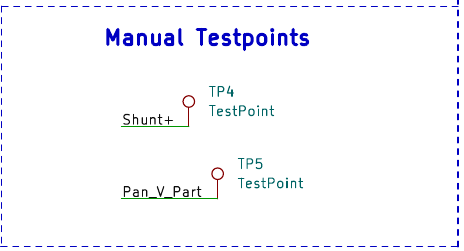
\includegraphics[scale=0.8]{figures/image70.png}
\captionsetup{type=figure}
\captionof{figure}{Testpoint per la misura manuale di tensione e corrente del pannello}
\end{center}

\hypertarget{actuation}{%
\section{Actuation}\label{actuation}}

\begin{center}
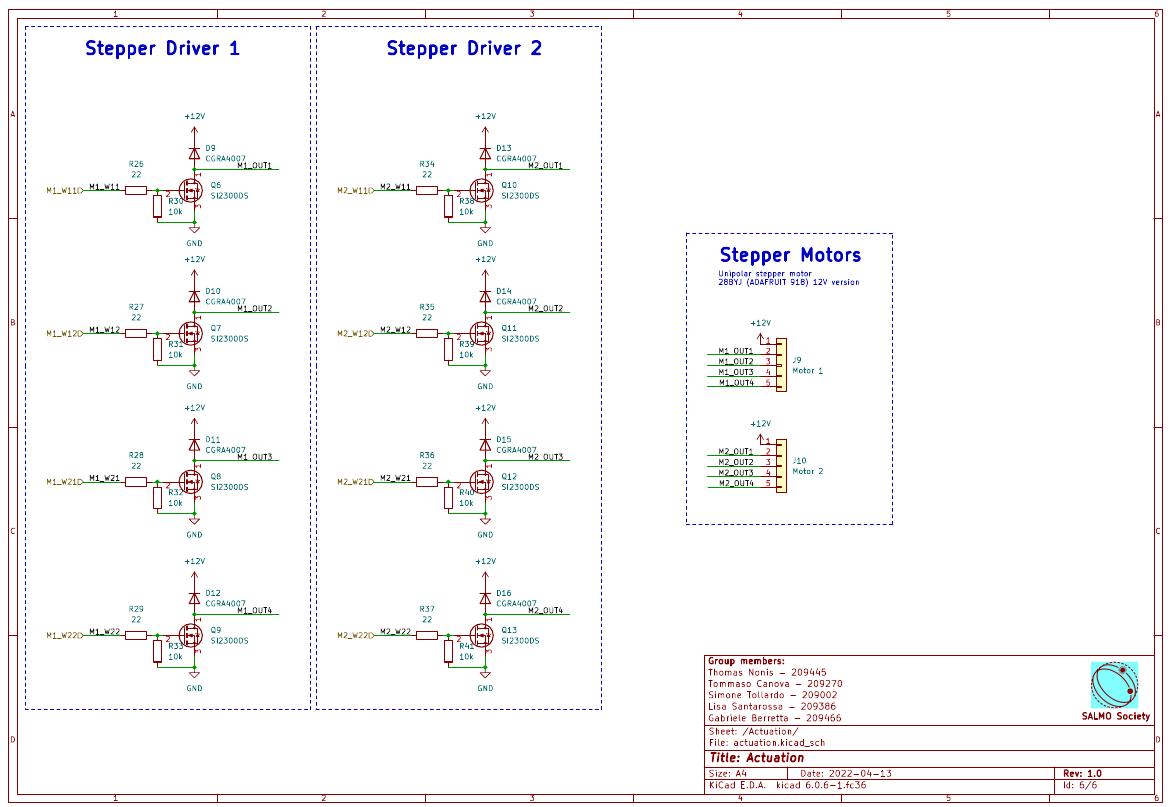
\includegraphics[width=6.5in,height=4.48611in]{figures/image41.png}
\captionsetup{type=figure}
\captionof{figure}{Foglio "Actuation" SALMO\newline}
\end{center}

La pagina dello schematico chiamata \emph{Actuation} prevede il comando
di due motori stepper unipolari tramite driver separati a
componentistica discreta e i relativi connettori. I due attuatori hanno
la funzione di orientare il pannello fotovoltaico nella direzione
desiderata, ruotando il pannello attorno agli assi \emph{z} e \emph{y}.

Abbiamo scelto i motori passo-passo \emph{Adafruit 918}, con tensione e
corrente nominali rispettivamente di 12V e 500mA, unipolari con
motoriduttore e coppia statica di 250gr/cm.

Da evidenziare è la presenza del motoriduttore (\emph{gearbox}) che
permette di ottenere una maggiore risoluzione (da 200 step fino a ben
512) e soprattutto una \emph{maggior coppia statica}; quest'ultima ci
consente di mantenere in posizione il pannello anche quando il motore è
disalimentato così da limitare i consumi totali. Ipotizzando, infatti,
il peso medio di un pannello fotovoltaico da 1W disponibile in commercio
di circa 20gr, una coppia statica di 250gr/cm risulta sufficiente per
consentire di ancorare meccanicamente a dovere il pannello all'asse del
motore.

\hypertarget{section-4}{%
\subsubsection{}\label{section-4}}

Per giunta, ogni motore essendo di tipo unipolare è dotato di due
avvolgimenti separati con presa intermedia comune pertanto sono
sufficienti solo quattro transistor per il comando del singolo. Infatti
a differenza degli stepper bipolari, non è necessario un \emph{h-bridge}
per cambiare il senso di rotazione ma basta invertire l'ordine
sequenziale di attivazione dei transistor. A seguito è illustrato il
circuito base a confronto:

\begin{center}
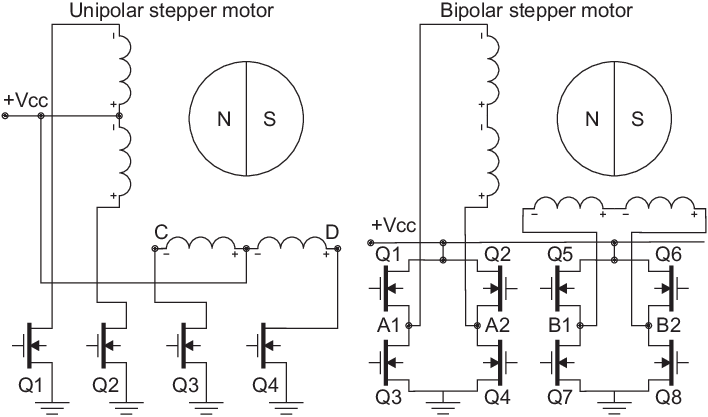
\includegraphics[scale=0.6]{figures/image75.png}
\captionsetup{type=figure}
\captionof{figure}{Driver per stepper unipolare vs driver per stepper bipolare\newline}
\end{center}

Il driver consiste nel porre in serie ad ogni fase del motore un n-mos
pilotato dal MCU, con resistenza di terminazione da 10kΩ e resistenza di
limitazione da 22Ω. La prima funge da pull-down nel caso in cui il pin
del MCU sia flottante, al fine di evitare accensioni involontarie del
transistor, pertanto abbiamo scelto il valore di 10kΩ analogamente alle
altre resistenze di pull-up/down già presenti nel circuito. Invece, la
resistenza da 22Ω limita la corrente sul ramo che connette il pin I/O al
gate del mosfet introducendo un ritardo nel fenomeno di carica e scarica
della capacità di gate-source del dispositivo, evitando così di bruciare
il pin del MCU dato che all'inserzione questa corrente può essere
elevata. Il valore di 22Ω è stato scelto arbitrariamente e fa sì che sul
gate del transistor ci sia una tensione di circa 3.3V (considerando il
partitore tra R26 e R27) quando il pin di output del microcontrollore è
a livello logico alto e, inoltre, determina una costante di
carica/scarica della capacità di ingresso di Q6 di:

\(\backslash tau = R\_\{ 26\}\ \backslash cdot\ C\_\{ gate - source\} = \ 22\backslash Omega\ \backslash cdot\ 7.3nF\ \backslash approx\ 160ns\)\(\)

Una costante di tempo di tale grandezza è considerata accettabile,
perchè ipotizzando una frequenza di lavoro dei mosfet di circa 20Hz,
quindi con un periodo di 55ms, permette allo switch di commuttare come
previsto.

In parallelo alle sezioni di avvolgimenti abbiamo inserito un diodo di
flyback cosicché all'apertura dello switch non si verifichino spike di
tensione critici tra drain e source dello stesso.

\begin{center}
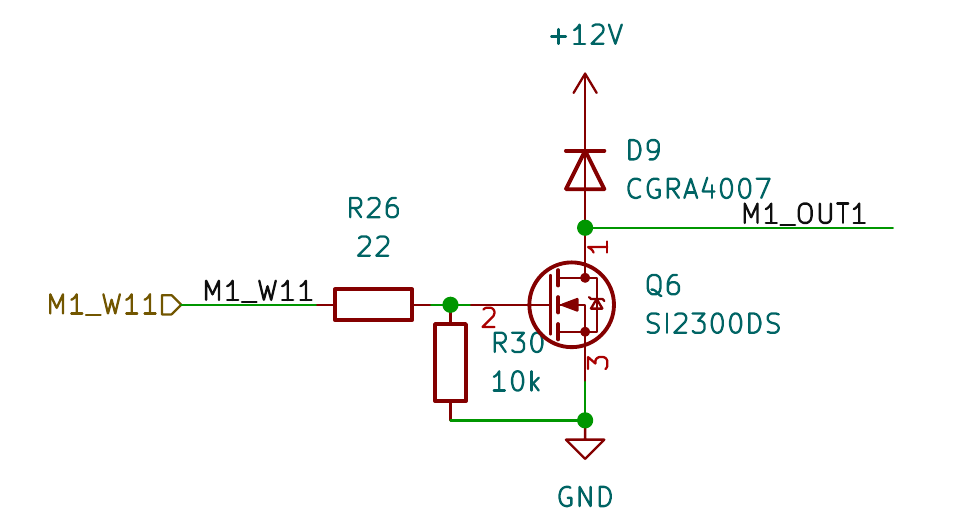
\includegraphics[scale=0.5]{figures/image63.png}
\captionsetup{type=figure}
\captionof{figure}{Circuito driver per un avvolgimento\newline}
\end{center}

Nel circuito in questione lo switch deve garantire:

\begin{enumerate}
\def\labelenumi{\arabic{enumi}.}
\item
  \begin{quote}
  di poter essere pilotato con una tensione di gate di almeno 3.3V
  (livello logico alto dei GPIO del MCU scelto);
  \end{quote}
\item
  \begin{quote}
  una corrente di drain di almeno 0.5A (corrente nominale dei motori);
  \end{quote}
\item
  \begin{quote}
  una differenza di potenziale tra drain e source di almeno 12V
  (tensione di alimentazione dei motori).
  \end{quote}
\end{enumerate}

Considerando le specifiche appena elencate abbiamo scelto dei transistor
Vishay SI2300DS nel comune package SOT23, con tensione di soglia 1.5V e
valori massimi supportati tra drain e source di 30V, tra gate e source
di 12V e una corrente di 3A.

\begin{center}
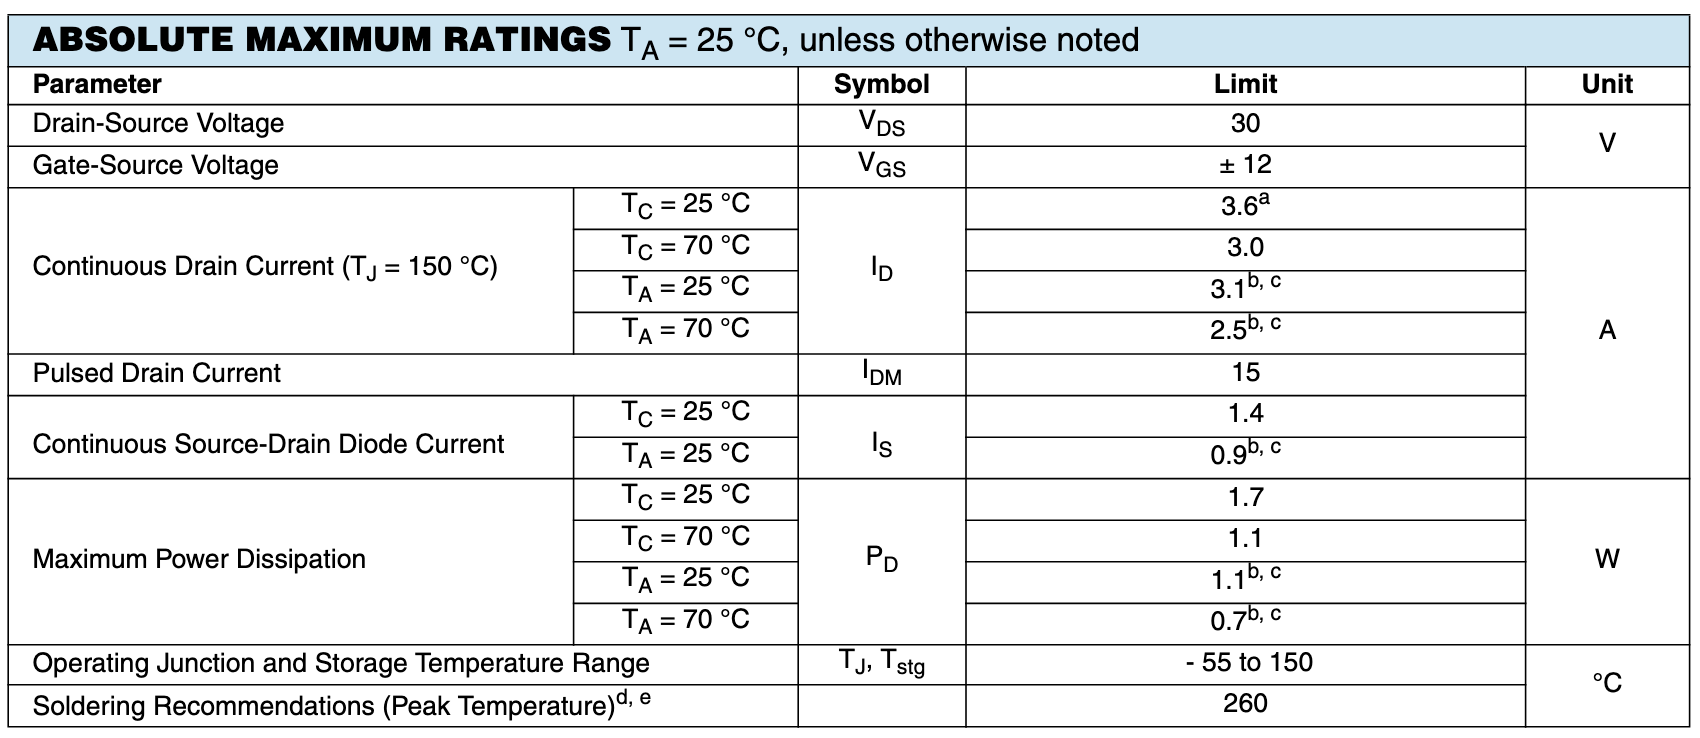
\includegraphics[scale=0.5]{figures/image69.png}
\captionsetup{type=figure}
\captionof{figure}{Estratto datasheet SI2300DS}
\end{center}
\chapter{Analisi del Layout PCB}

Una volta terminato il progetto dello schematico e verificata la sua
correttezza, siamo passati allo sbroglio circuitale. Abbiamo quindi
esportato la netlist da \emph{eeschema} per poi importarla in
\emph{pcbnew}, popolando il progetto con i footprint di tutti i
componenti.

\hypertarget{layout}{%
\section{Layout}\label{layout}}

Come primo passo abbiamo raggruppato i vari componenti per sezione
circuitale (alimentazione, microcontrollore, controllo motori,
ecc\ldots) in modo da avere un primo ordine.\\
Fino a questo punto non abbiamo posto alcun riguardo verso la posizione
dei componenti, ma abbiamo semplicemente effettuato una suddivisione
funzionale. Con il passo successivo abbiamo invece collocato, per
ciascun blocco circuitale, ogni componente nel modo che più ci è
sembrato adeguato, tenendo in mente gli aspetti elettrici (per esempio
il posizionamento del GPS lontano dalla sezione di potenza e dal
microcontrollore), di distanziamento, di funzionalità (per esempio
posizionamento di connettori e pulsanti), di comodità per l'utente
finale ed infine di estetica.\\
Per quanto riguarda la sezione legata al microcontrollore abbiamo
posizionato, in ordine di priorità:

\begin{enumerate}
\def\labelenumi{\arabic{enumi}.}
\item
  
  il quarzo con i suoi condensatori ed il suo resistore il più vicino
  possibile ai pin \textit{XIN} e \textit{XOUT};
  
\item
  
  i condensatori di decoupling più vicini possibile ai pin di
  alimentazione;
  
\item
  
  la memoria flash;
  
\item
  
  i resistori di terminazione della linea USB.
  
\end{enumerate}

\begin{center}
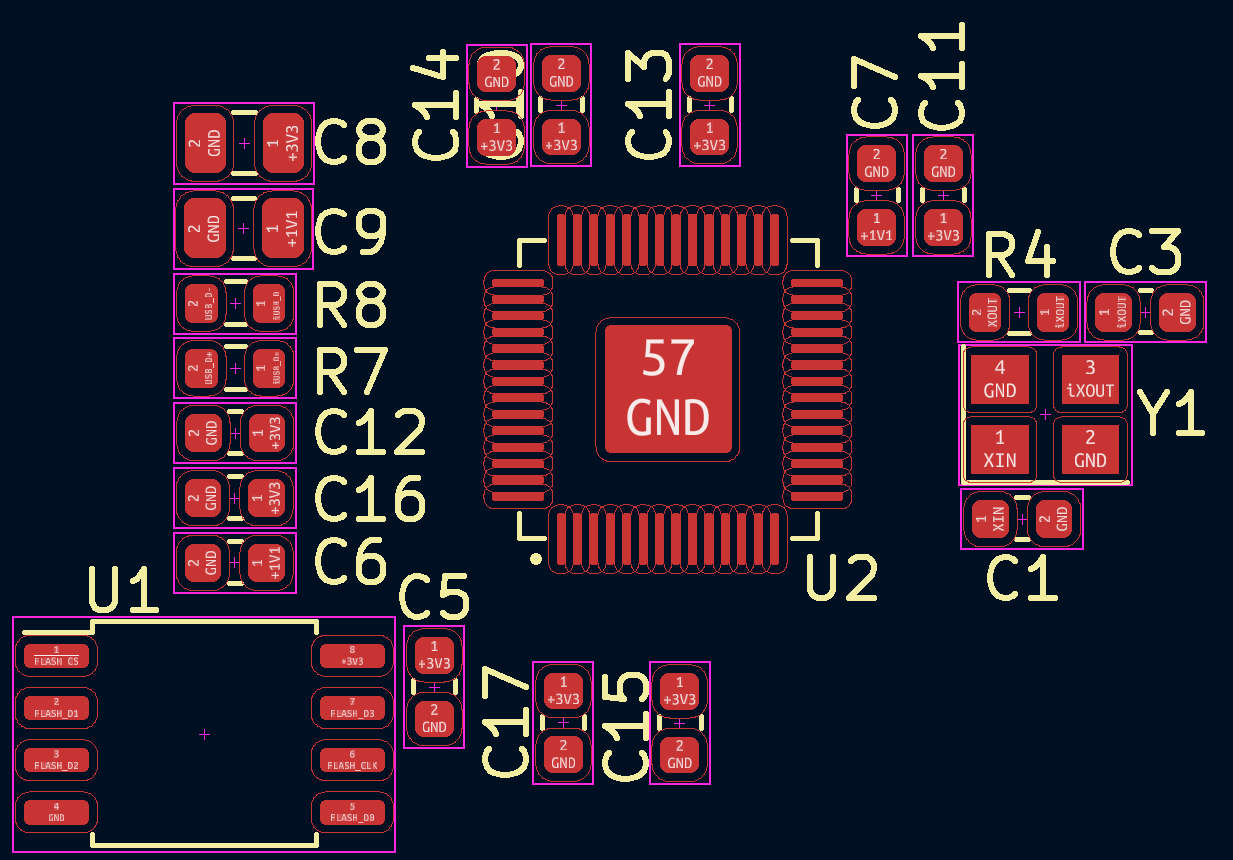
\includegraphics[scale=0.3]{figures/image29.png}
\captionsetup{type=figure}
\captionof{figure}{Primo posizionamento componenti principali foglio Control}
\end{center}

\noindent Il fatto di posizionare i componenti il più vicino possibile ai relativi
pin è necessario per ridurre di quanto possibile l'impedenza della linea
di alimentazione, e quindi la lunghezza del percorso del segnale.
Maggiore è la lunghezza del percorso tra condensatore e pin e maggiore
sarà l'induttanza parassita della traccia, che porta a problemi di
integrità di segnale quando si ha a che fare con segnali ad alta velocità.
Considerando a titolo di esempio una linea di alimentazione,
l'induttanza parassita è contrastata dalla presenza dei condensatori di
decoupling. In questo modo siamo in grado fornire un percorso a bassa
impedenza tra condensatore e pin del MCU, perciò la restante lunghezza
che va dal condensatore al pin di alimentazione deve rimanere il più
breve possibile. Si noti che ai fini del calcolo si deve considerare sia
la linea di andata (es: alimentazione) che quella di ritorno (GND).\\
Per quanto riguarda la sezione di controllo dei motori abbiamo
posizionato i connettori, i transistor, i diodi ed i resistori di
polarizzazione in modo da ridurre al minimo le tracce necessarie e da
allineare il tutto per renderlo il più esteticamente bello possibile.

\begin{center}
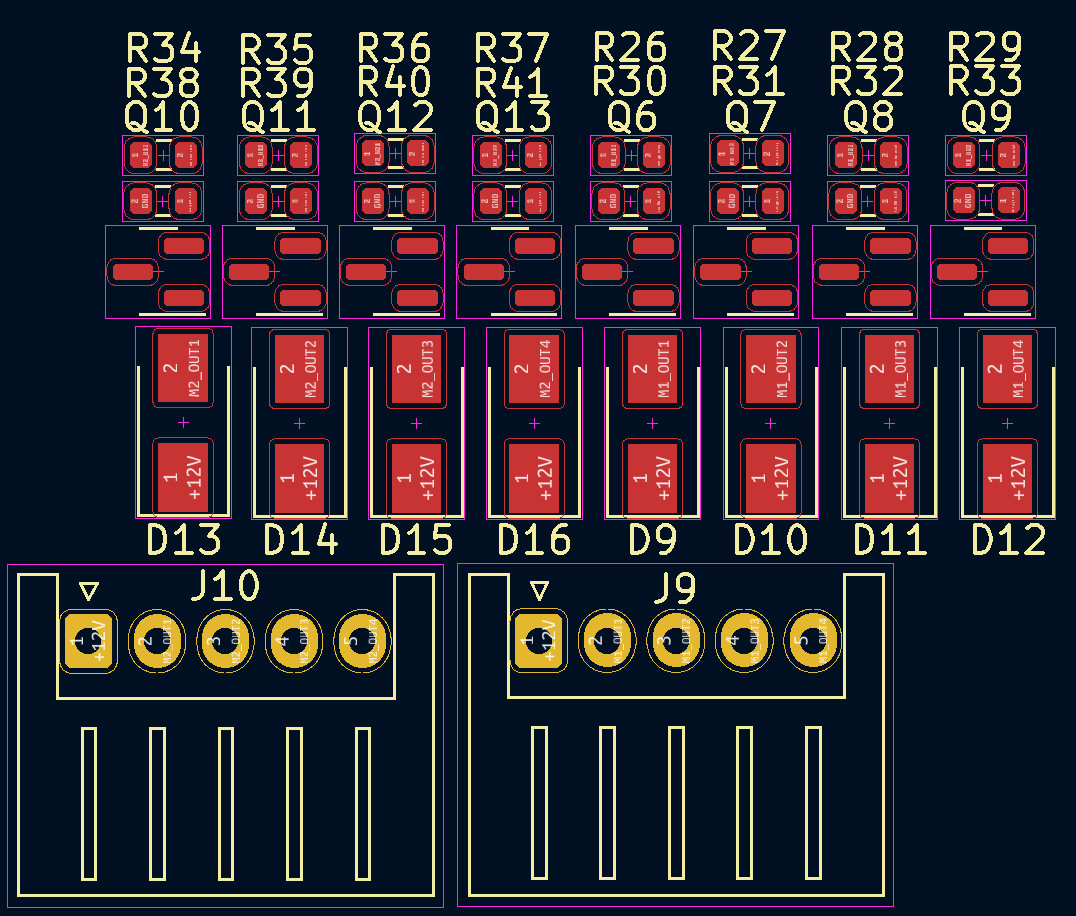
\includegraphics[scale=0.3]{figures/image55.png}
\captionsetup{type=figure}
\captionof{figure}{Primo posizionamento componenti driver motori stepper}
\end{center}

\noindent Parlando dello stadio di alimentazione, abbiamo posizionato tutti i
componenti in modo da minimizzare il numero di tracce necessarie e da
facilitare il routing di tracce di grande spessore. Abbiamo rivolto
particolare attenzione al regolatore a commutazione, cercando di rendere
il nodo di switching più piccolo possibile per ridurre al minimo il
\textit{ripple}.

\begin{center}
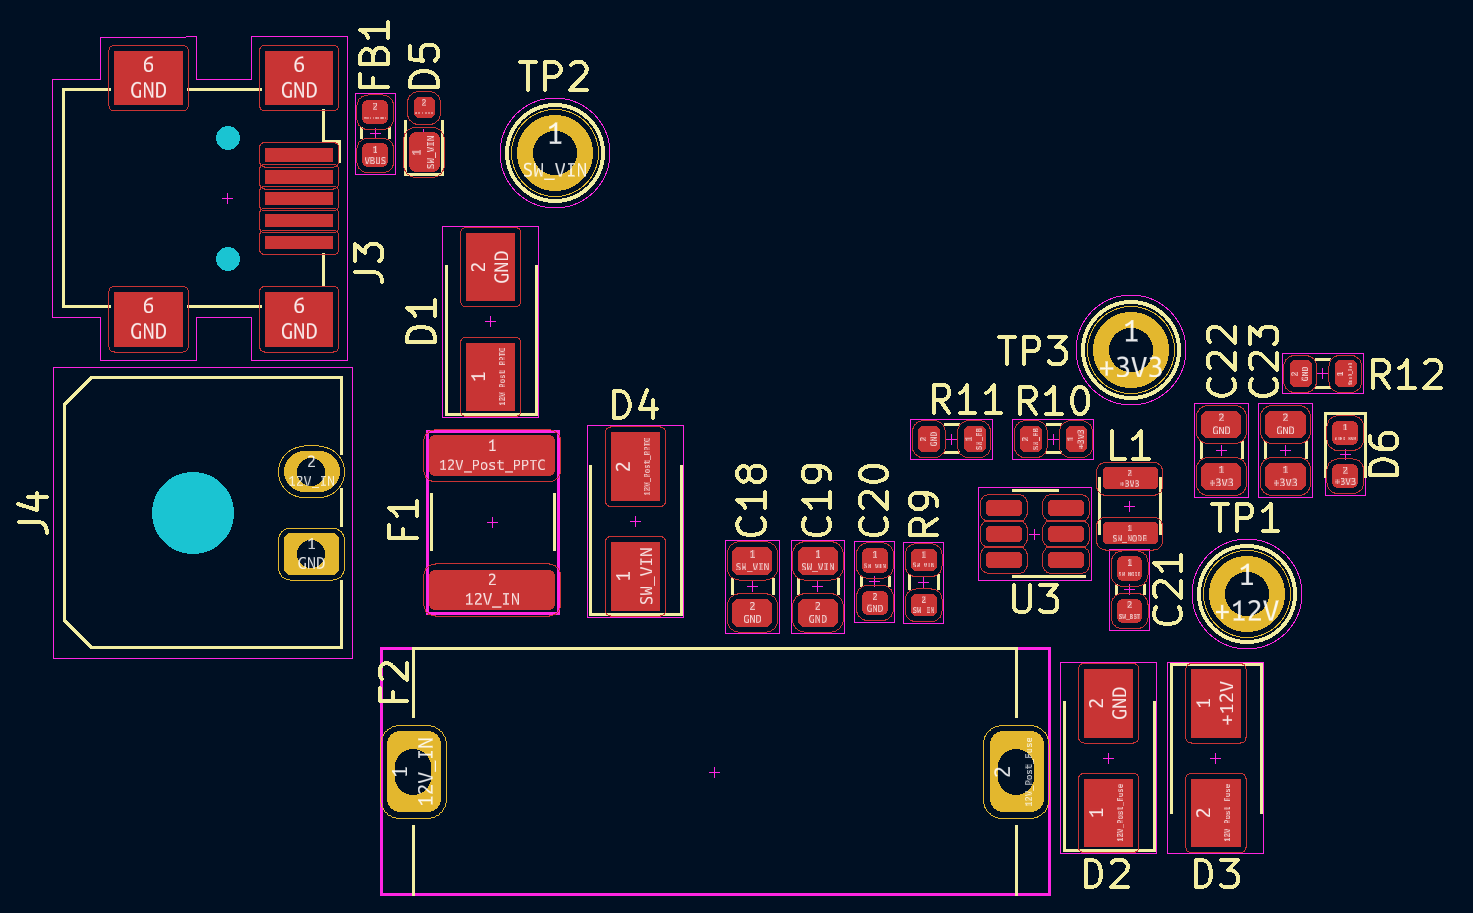
\includegraphics[width=0.5\textwidth]{figures/image56.png}
\captionsetup{type=figure}
\captionof{figure}{Primo posizionamento componenti foglio Power}
\end{center}

\noindent Le restanti sezioni non includono componenti particolarmente critici,
quindi il posizionamento è stato fatto seguendo il principio di
semplicità di routing delle tracce e di bellezza estetica.\\
A questo punto, dopo aver ottenuto un insieme di diversi blocchi
circuitali, abbiamo provato a posizionarli in modo da capire che
dimensioni imporci come limite per la scheda ed abbiamo appurato che
100x60mm fosse una misura adeguata per contenere il tutto.\\
Avendo definito le dimensioni siamo passati alla creazione del disegno
del contorno della scheda sul layer \textit{Edge.Cuts}, introducendo un
arrotondamento degli angoli per fini puramente estetici. Successivamente
abbiamo disegnato i rettangoli di riempimento, assegnandoli alla net di
GND e con priorità minima per entrambi i layer, in modo che coprissero
la scheda intera.\\
Abbiamo quindi posizionato i blocchi circuitali discussi in precedenza,
non prima di aver posizionato i fori di montaggio ed i \textit{fiducials},
facendo in modo di avere i connettori lungo il bordo. Anche il \textit{GPS} è
stato posizionato in un angolo in modo da tenerlo il più lontano
possibile da ogni altro componente; sotto il suo ingombro abbiamo
inserito anche una \emph{keepout zone}, come richiesto da datasheet.

\begin{center}
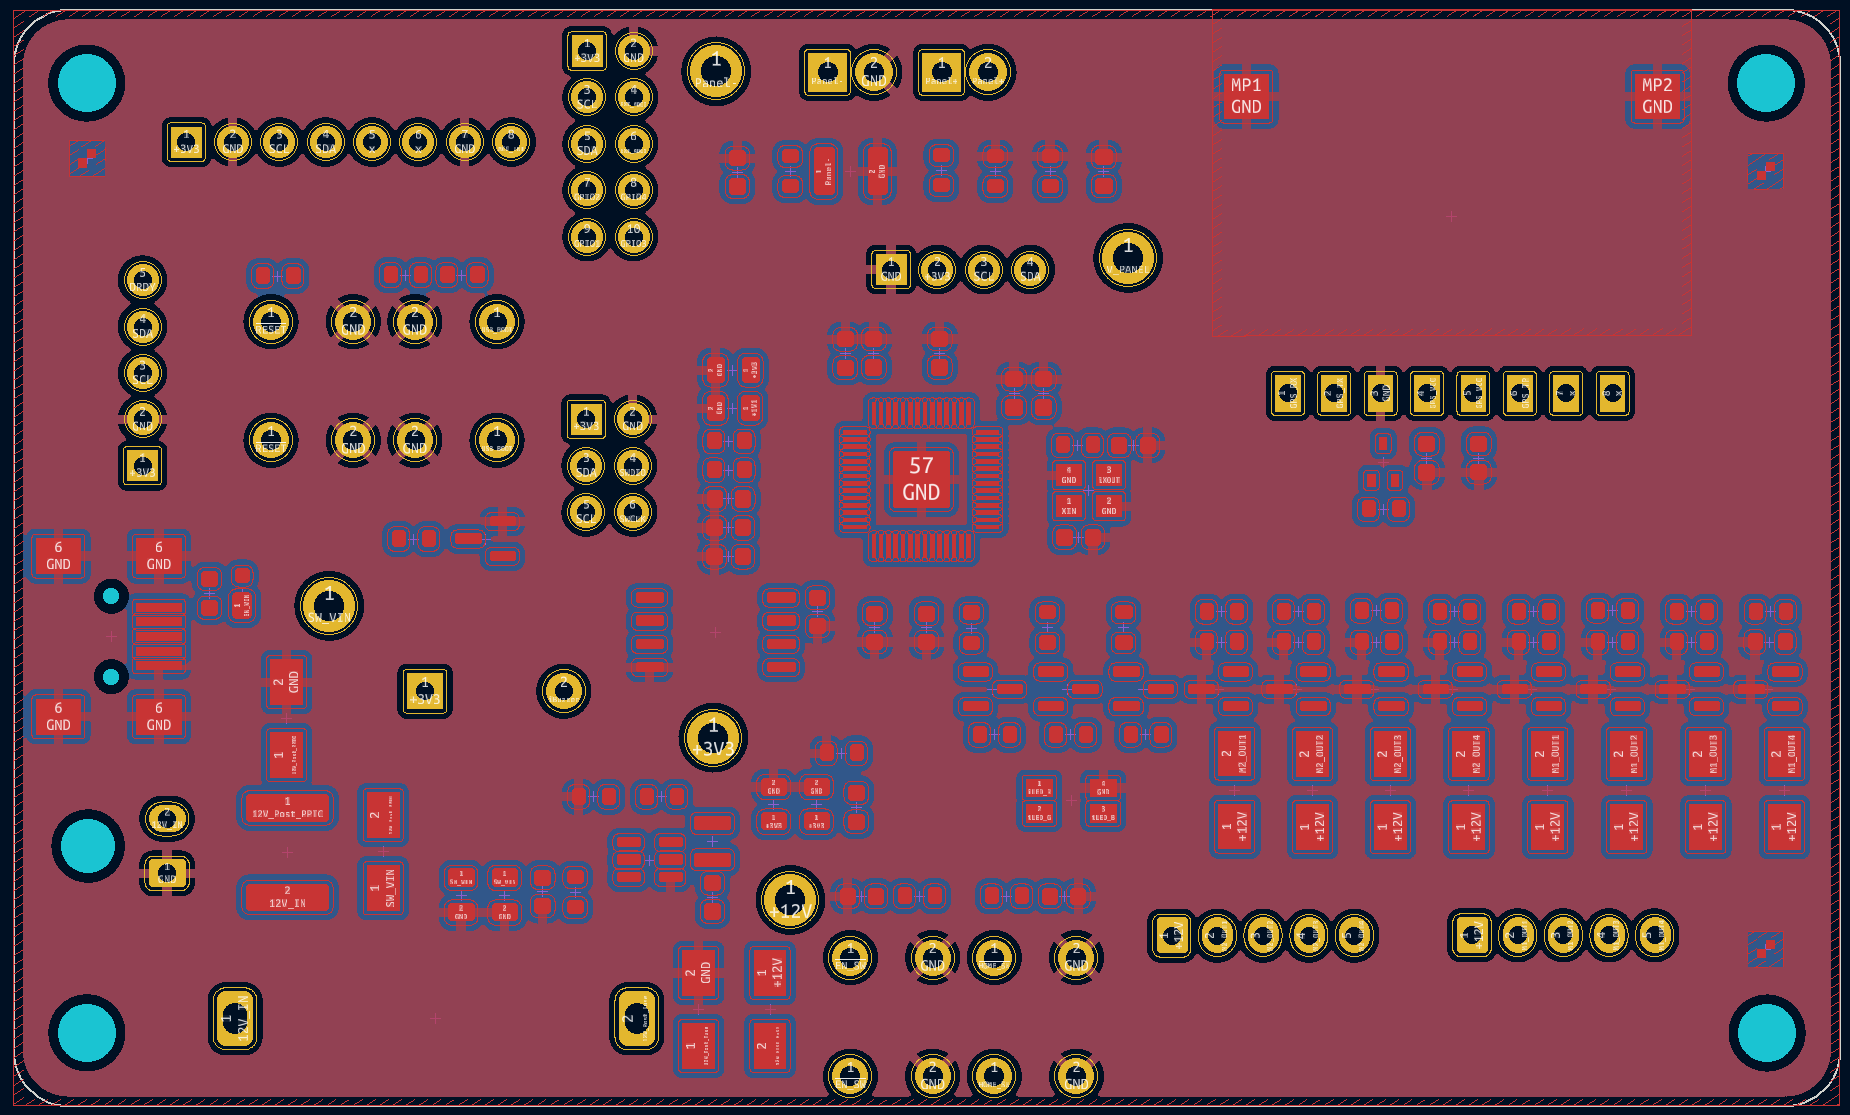
\includegraphics[width=4.57535in,height=2.75694in]{figures/image21.png}
\captionsetup{type=figure}
\captionof{figure}{Prima bozza piazzamento componenti}
\end{center}

\hypertarget{routing}{%
\section{Routing}\label{routing}}

\noindent Una volta definite le posizioni dei vari componenti siamo passati alla
fase di routing, cominciando dalle linee particolarmente sensibili e poi
quelle di alimentazione. Prima di iniziare abbiamo creato una serie di
dimensioni predefinite per le tracce:

\begin{itemize}
\item
  
  0.2mm per il \textit{fanout} del microcontrollore
  
\item
  
  0.3mm per le linee di segnale in generale
  
\item
  
  0.5mm per le linee di alimentazione
  
\item
  
  0.8mm per le linee di alimentazione dei motori
  
\end{itemize}

\noindent Abbiamo inoltre creato due dimensioni predefinite per le \textit{vias} (diametro
pad/diametro foro):

\begin{itemize}
\item
  
  0.55mm/0.25mm per le linee di segnale
  
\item
  
  0.8mm/0.4mm per le linee di alimentazione
  
\end{itemize}

\noindent Una volta preparato l'ambiente di lavoro abbiamo cominciato a collegare
tutte le linee di alimentazione, partendo prima da quelle più corte che,
per esempio, collegano un pin di un dispositivo al relativo condensatore
di decoupling, per effettuare solo alla fine i collegamenti più lunghi
facendo in modo di lasciare sufficiente spazio per le linee di segnale.\\
Per quanto riguarda il routing dell'alimentazione vogliamo sottolineare
3 accorgimenti che abbiamo preso:

\begin{itemize}
\item
  
  per le tracce che vanno dal connettore del pannello solare allo shunt
  per misurare la corrente, abbiamo deciso di utilizzare uno spessore di
  1mm, in modo da ridurne al minimo la resistenza;
  
\item
  
  per effettuare il fanout del microcontrollore abbiamo utilizzato
  tracce da 0.2mm per allontanarsi dai pin, per poi allargarle il prima
  possibile a 0.3mm;
  
\item
  
  per il routing della linea di alimentazione a 12V per il controllo dei
  motori abbiamo utilizzato per quanto possibile i poligoni di
  riempimento, assegnando la net 12V ed impostando la priorità ad 1.
  
\end{itemize}

\begin{center}
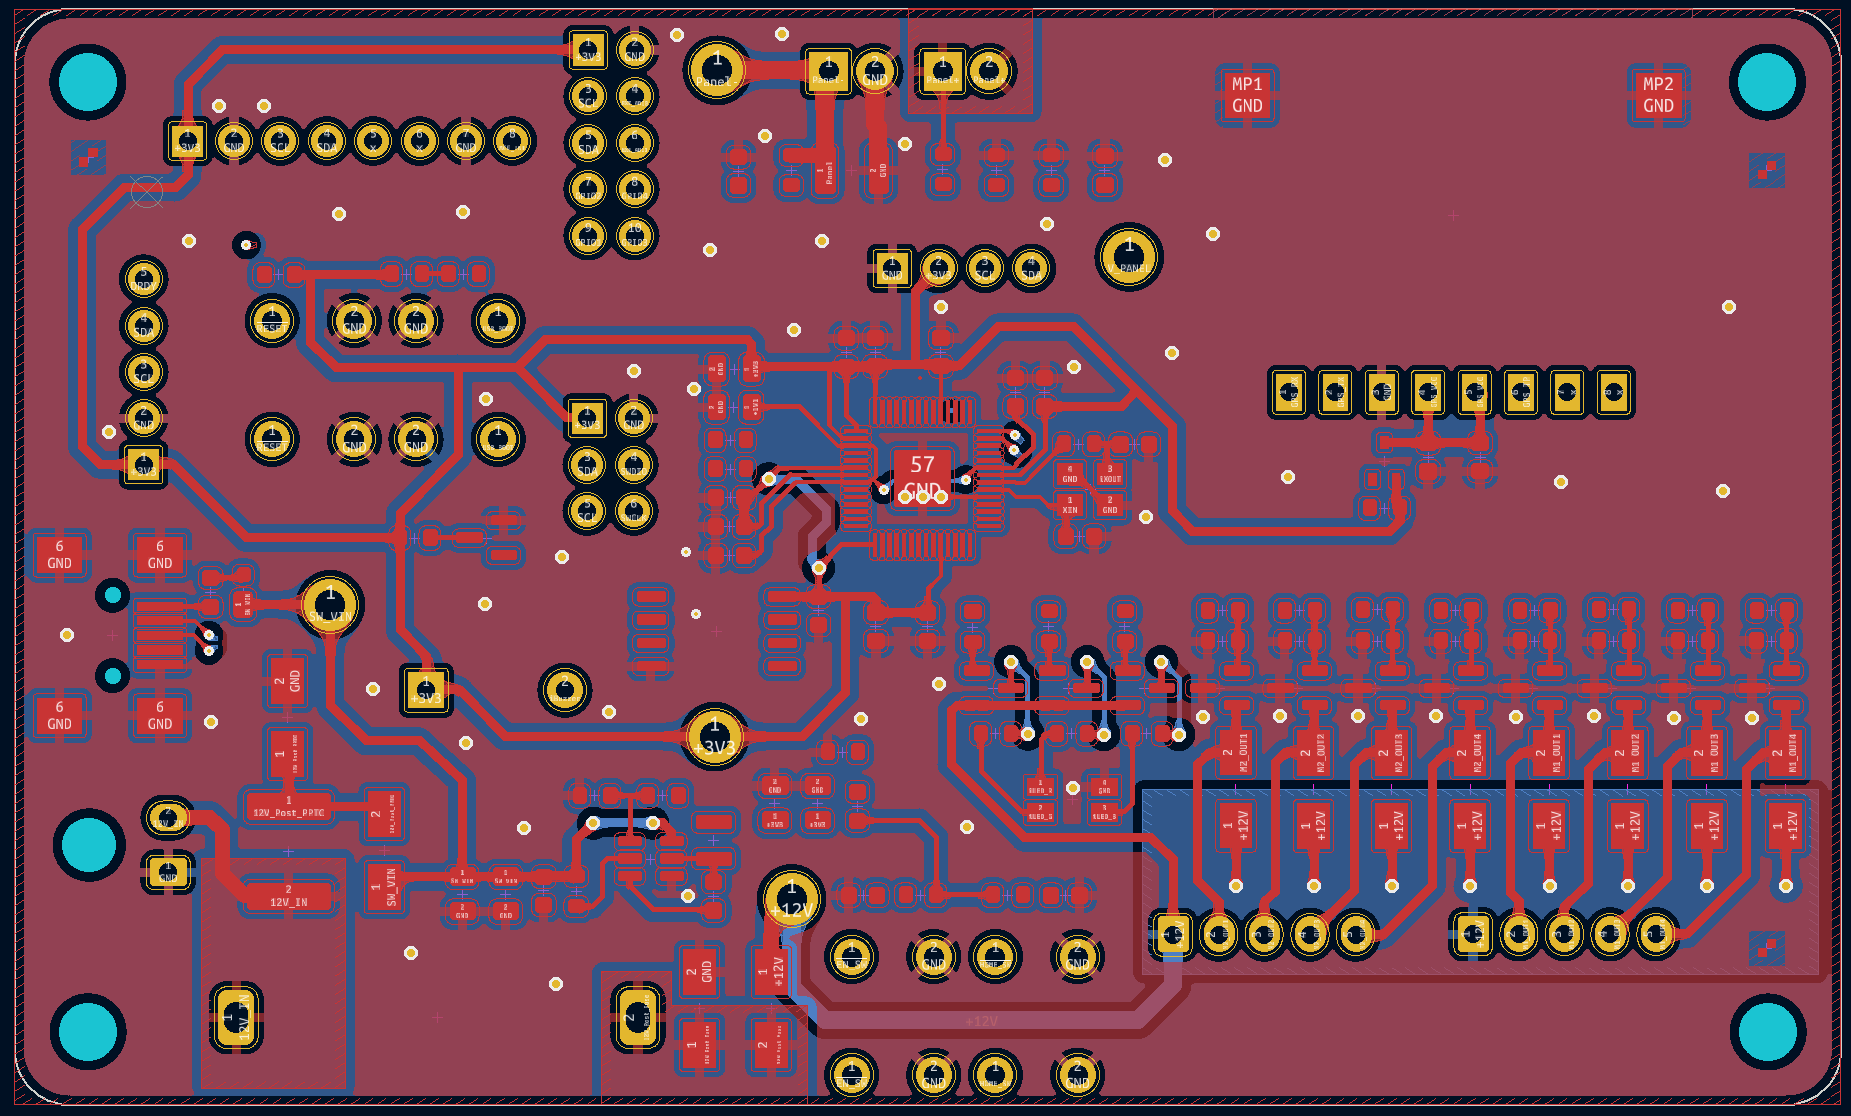
\includegraphics[scale=0.2]{figures/image77.png}
\captionsetup{type=figure}
\captionof{figure}{Prima bozza routing tracce}
\end{center}

\noindent Una volta concluso il routing delle linee di alimentazione siamo passati
alle restanti linee di segnale iniziando dal fanout del
microcontrollore, anche in questo caso partendo con tracce da 0.2mm per
poi allargarle a 0.3mm.\\
Abbiamo considerato per primi i segnali critici, ovvero le linee del
quarzo, quelle per la trasmissione \textit{QSPI} della flash e quelle
differenziali per l'USB. Sebbene non sia di apprezzabile effetto dal
punto di vista funzionale, abbiamo voluto provare, a titolo di esercizio
personale, il tool di \emph{length matching} per rendere le linee
differenziali D+ e D- dell'USB più simili possibile in termini di
lunghezza. Questo è stato fatto, perché abbiamo riscontrato alcune
difficoltà nell'utilizzo del router differenziale, che avrebbe gestito
il \emph{length matching} in autonomia.\\
Avendo definito le tracce critiche siamo poi passati al fanout e al
routing dei restanti segnali. Durante questo processo abbiamo iterato
più volte spostando le assegnazioni di alcuni pin del microcontrollore,
grazie alle matrici di assegnazione dei GPIO, in modo da trovare le
posizioni ottimali.\\
Questa parte dello sbroglio è stata la più complessa a causa della
necessità di avere molti dispositivi vicini al microcontrollore e alla
ridotta \emph{clearance} tra i pin.

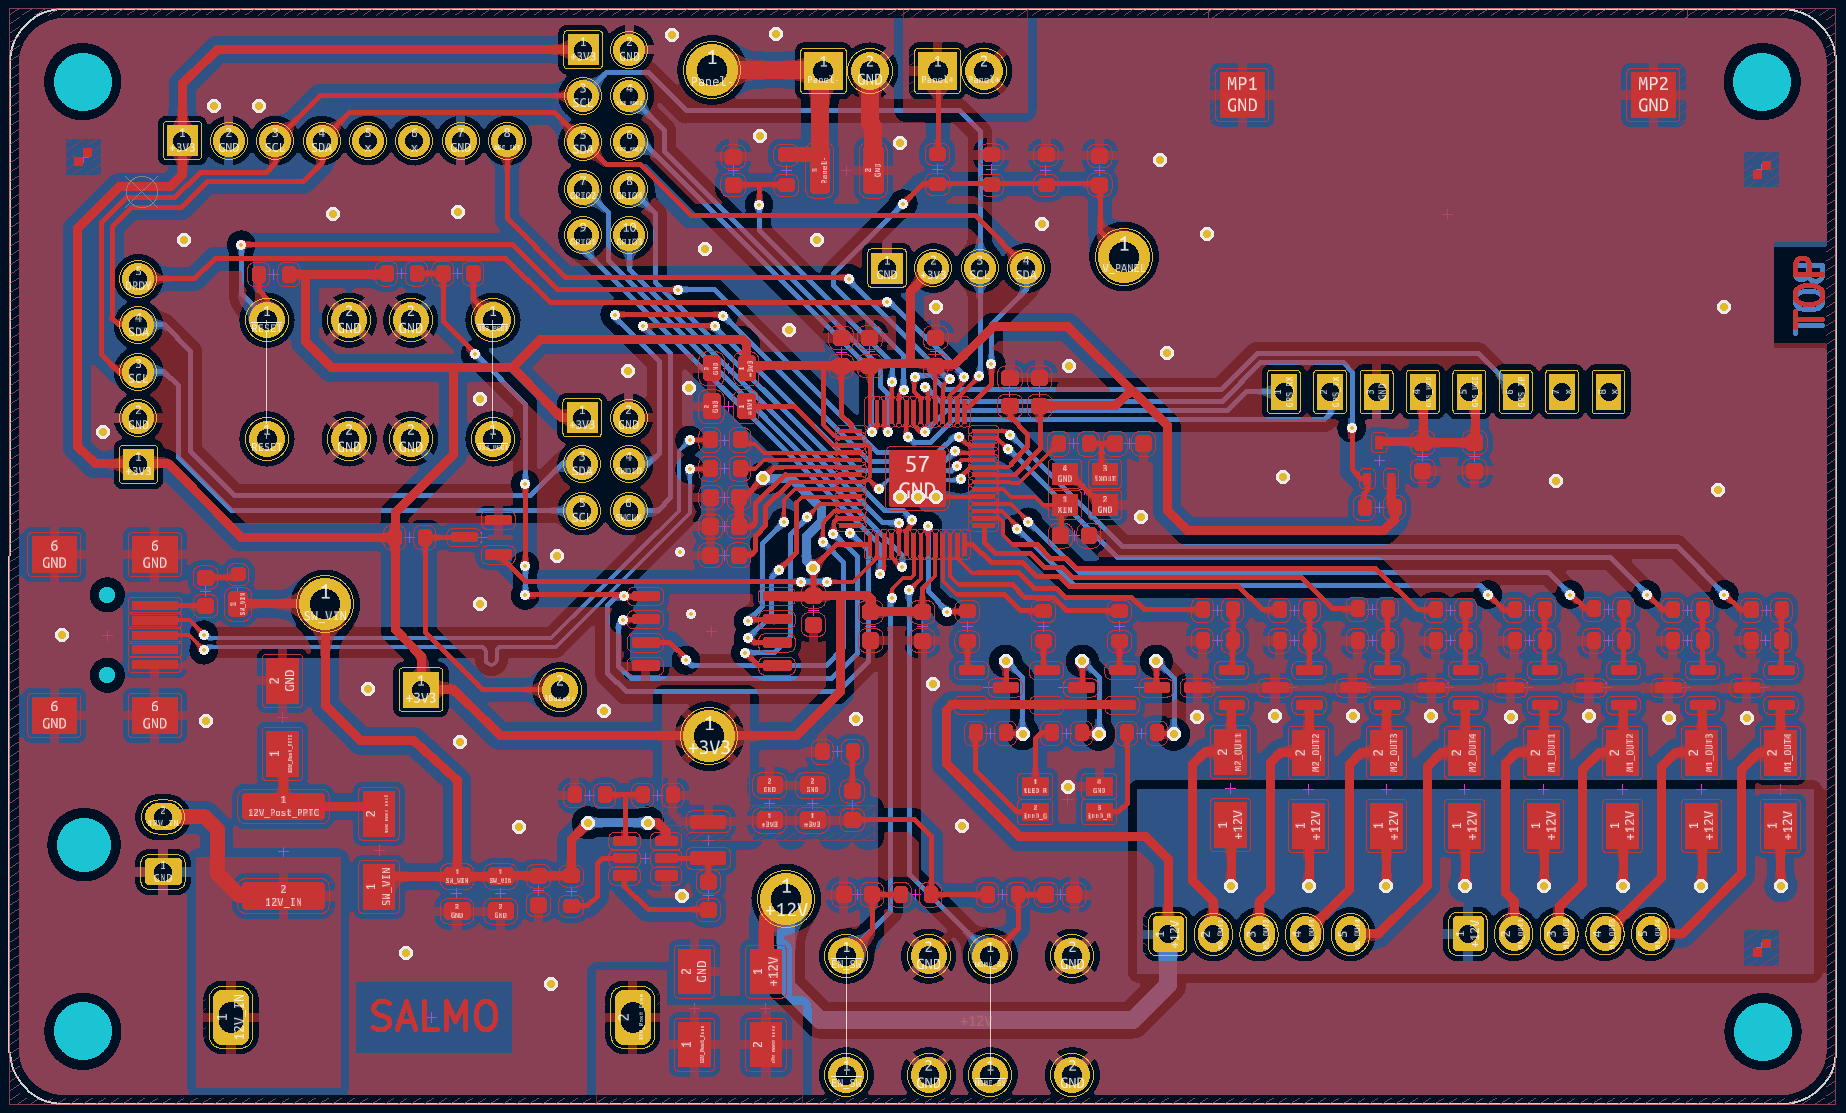
\includegraphics[scale=0.16]{figures/image59.png}
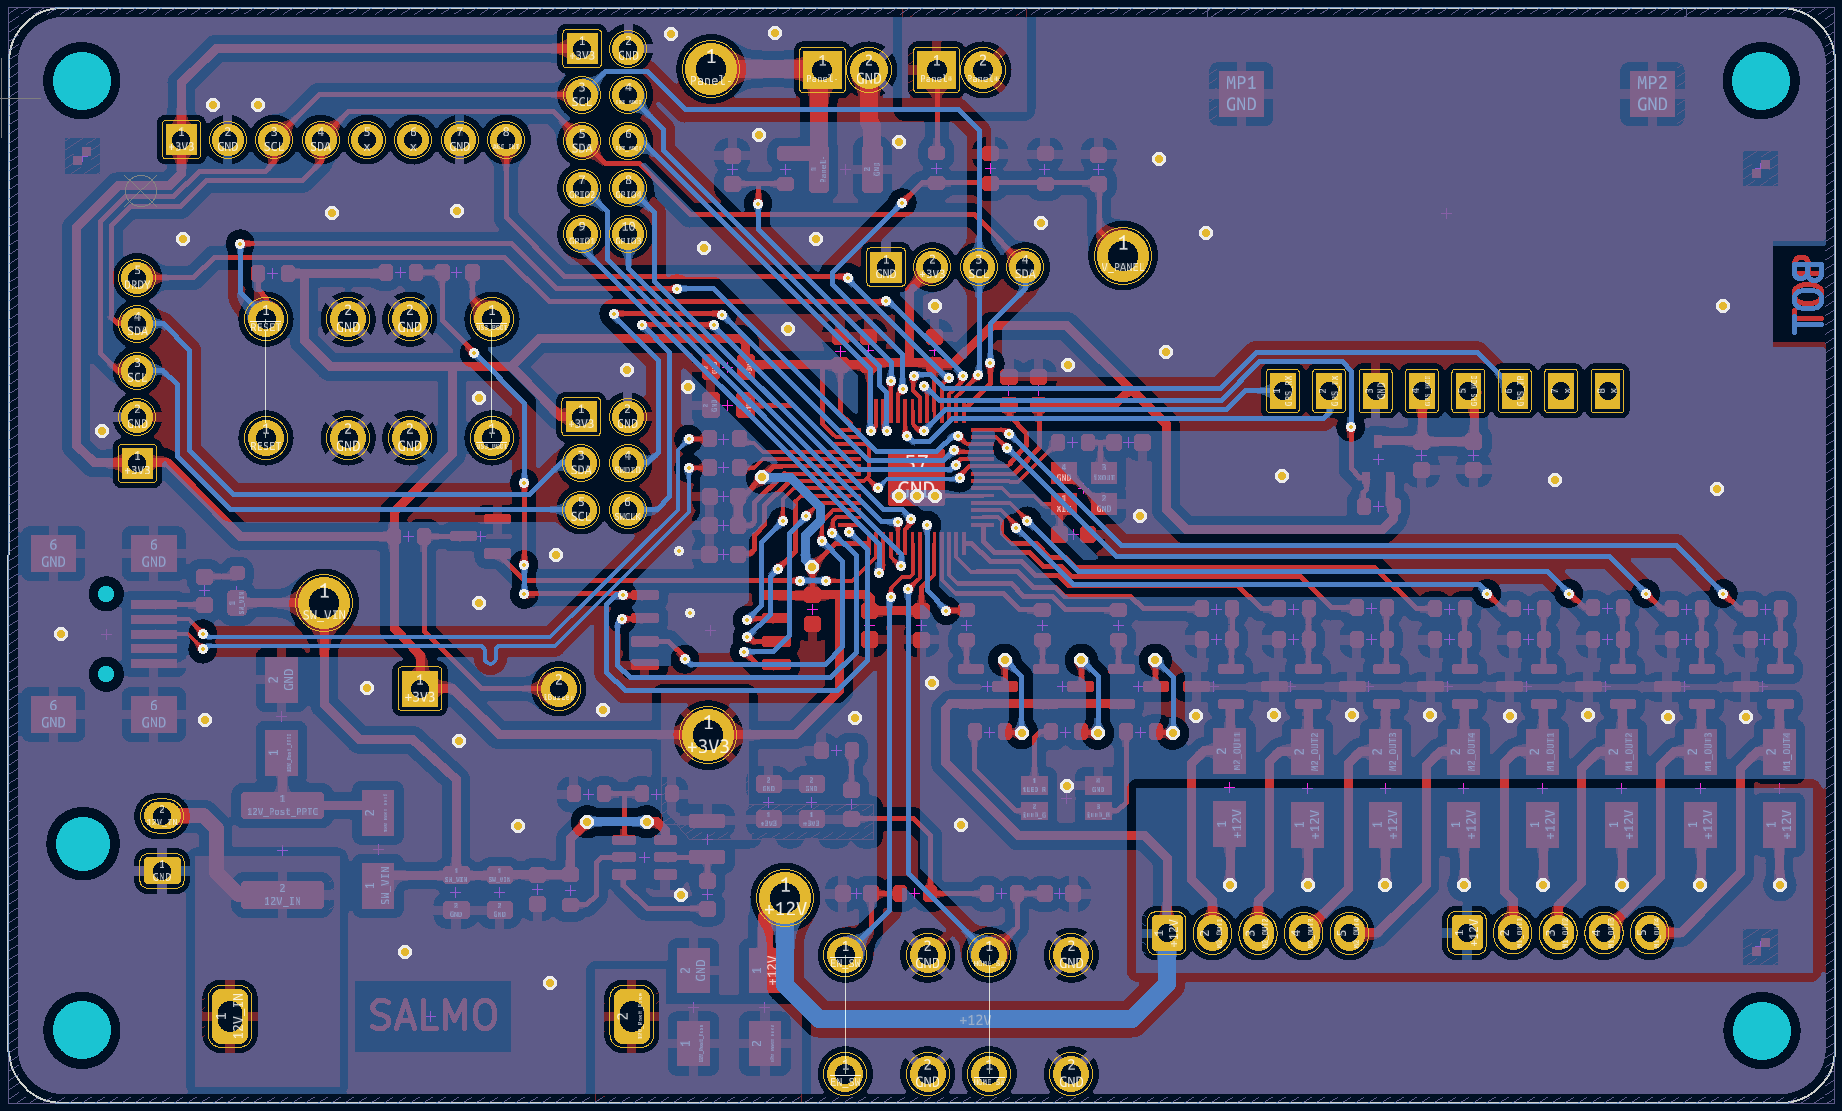
\includegraphics[scale=0.16]{figures/image22.png}
\begin{center}
\captionsetup{type=figure}
\captionof{figure}{Primo risultato routing PCB}
\end{center}

\noindent Terminato il routing di tutte le tracce abbiamo fatto un'analisi per
cercare eventuali sviste o errori commessi, sia facendo un'ispezione
visiva, sia utilizzando il \textit{DRC}. Prevedibilmente abbiamo riscontrato
qualche errore che abbiamo prontamente corretto senza troppe difficoltà.\\
Anche dopo queste correzioni il \textit{DRC} restituisce alcuni errori, che però
sono previsti e non causano problemi nella realizzazione. Questi sono di
due tipi, il primo è il \emph{Courtyards overlap} per i componenti che
stanno vicino al \textit{GPS}, mentre il secondo è l' \emph{Items not allowed} ed
è dovuto a come sono stati realizzati i footprint dei fiducials.\\
Il primo lo si può ignorare, perché in realtà il \textit{GPS} sarà montato su un
header rialzato e quindi la superficie del PCB sarà libera da
occlusioni. Il secondo errore invece è dovuto al fatto che il footprint
dei \textit{fiducials} è stato realizzato con due pad che sovrappongono una
\emph{keepout zone}, questo però è comunque un effetto desiderato,
quindi possiamo ignorarlo.

\hypertarget{finitura}{%
\section{Finitura}\label{finitura}}

\noindent Arrivati a questo punto abbiamo appurato che l'aspetto elettrico della
scheda era corretto, quindi ci siamo concentrati sugli aspetti estetico
e utilitario.\\
Prima di tutto abbiamo aggiunto un pad di GND a lato scheda per poter
collegare una pinza a coccodrillo in modo da semplificare le misurazioni
per il debug hardware. Poi abbiamo fatto in modo di posizionare, sul
layer \textit{silkscreen} tutti i \textit{refdes} dei componenti, in modo tale che fossero
ordinati e ben visibili, facendo particolare attenzione, per quanto
possibile, a non posizionarli sopra vias che avrebbero causato
potenziali problemi di lettura.

\begin{center}
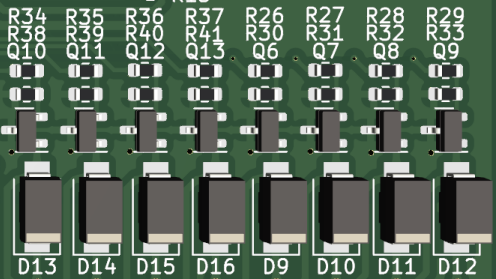
\includegraphics[width=0.5\textwidth]{figures/image100.png}
\captionsetup{type=figure}
\captionof{figure}{Esempio Silkscreen SALMO}
\end{center}

\noindent Sistemati tutti i \textit{refdes} abbiamo aggiunto sui layer di \textit{silkscreen}
ulteriori descrizioni per chiarire le funzioni dei connettori e per
aggiungere informazioni utili. In particolare abbiamo aggiunto 
l’indicazione di polarità sul connettore di alimentazione e, ad ogni
connettore il suo nome e, sul retro, la descrizione di ogni pin. Per i
connettori di espansione e debug non c'era spazio a sufficienza, quindi
abbiamo creato sul retro una grafica apposita composta da una tabella,
che rappresenta la funzione di ogni pin, e da un segmento di retta che
riconduce la tabella al connettore a cui fa riferimento.\\
Abbiamo successivamente aggiunto, sempre sul retro, il titolo del
progetto con il nome del corso, nomi, cognomi e matricole dei membri del
gruppo e data e numero di revisione.

\begin{center}
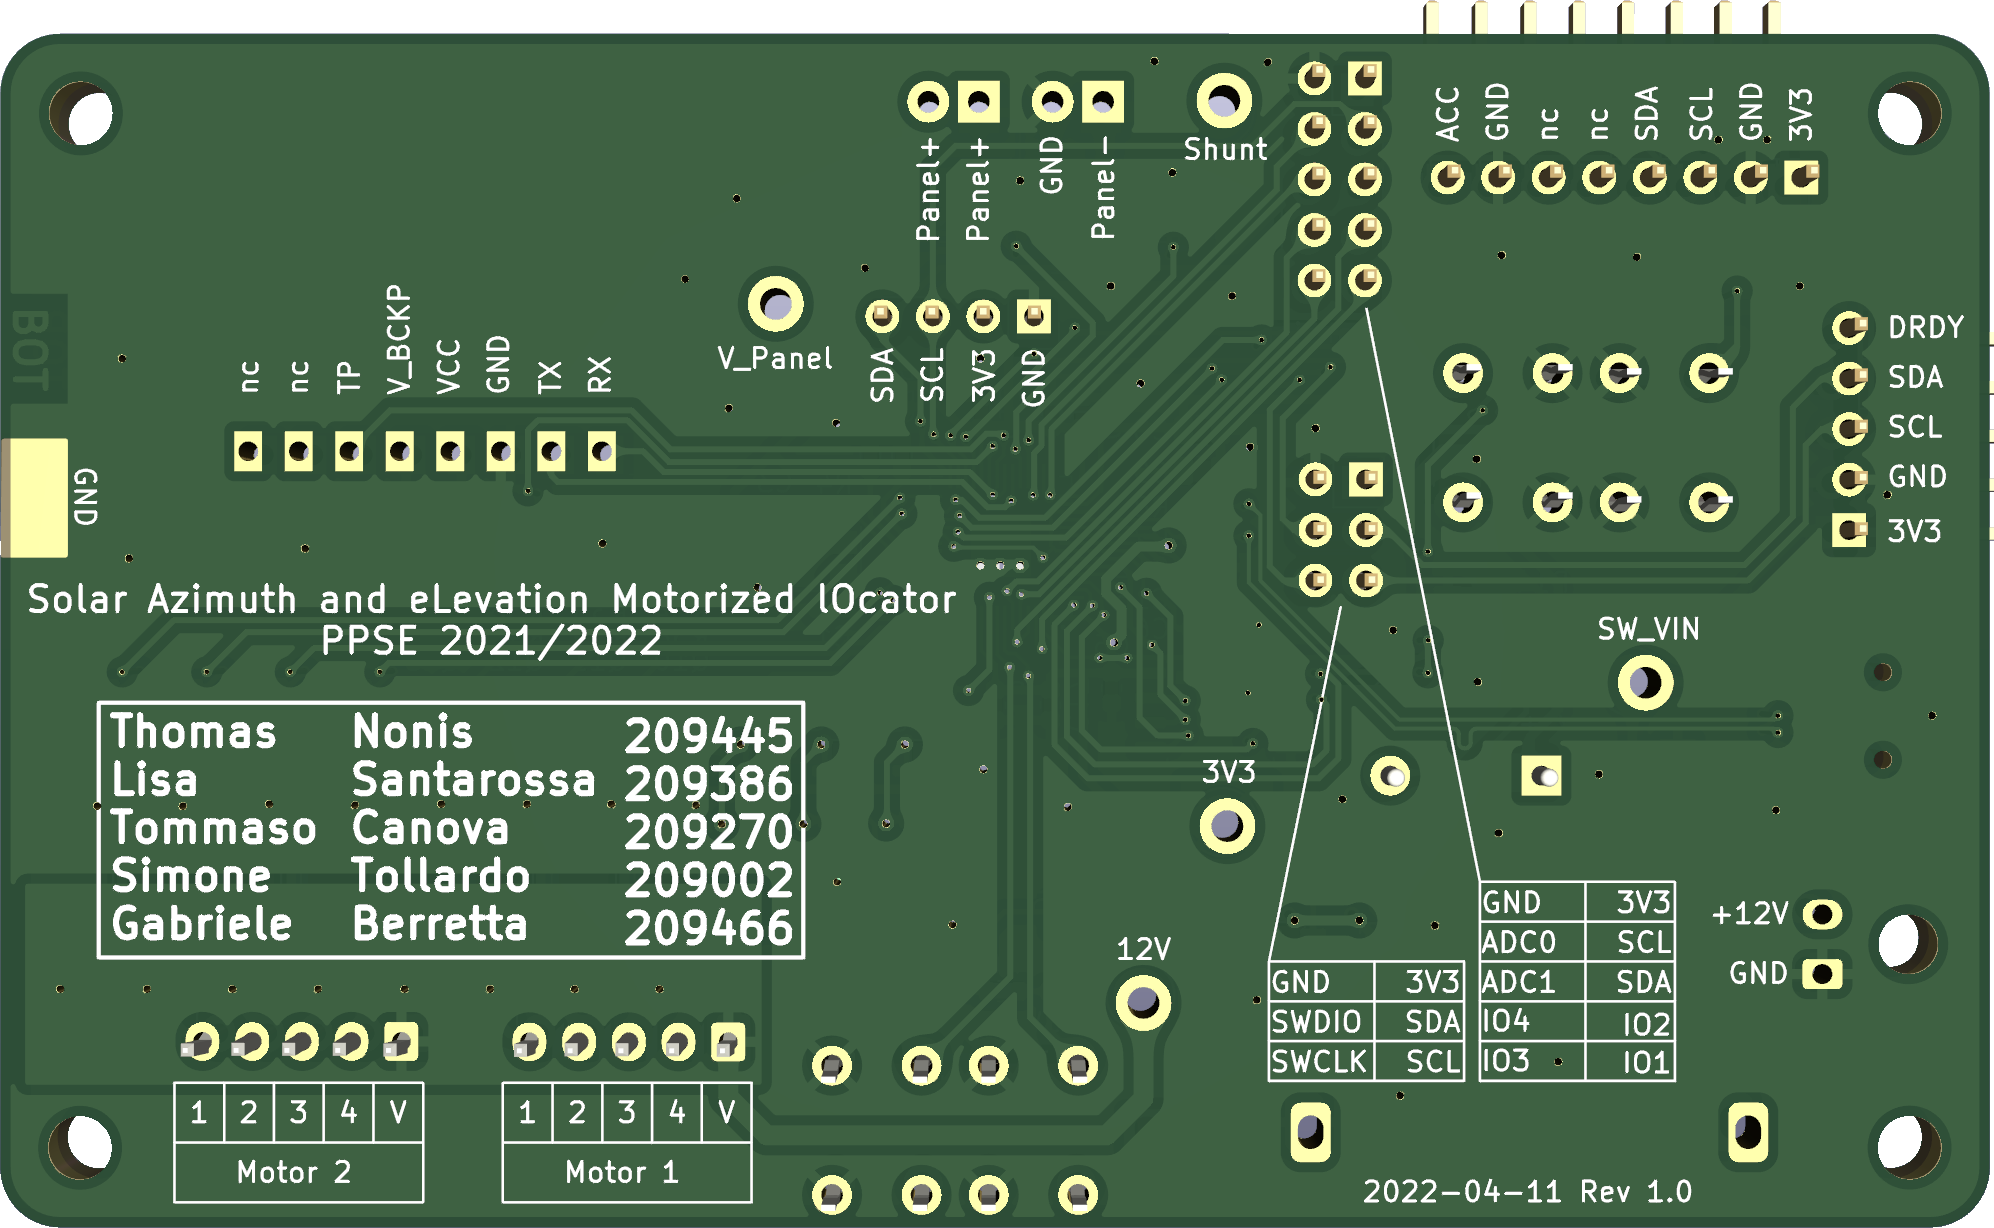
\includegraphics[scale=0.2]{figures/image42.png}
\captionsetup{type=figure}
\captionof{figure}{Vista del retro della PCB SALMO}
\end{center}

\noindent Per poter facilmente identificare i layer \textit{top} e \textit{bottom} abbiamo aggiunto,
a lato scheda, i testi TOP e BOT sui layer corrispondenti.\\
A questo punto la scheda si può considerare terminata e non è rimasto
altro da fare che generare i \textit{teardrops}, tramite un plugin dedicato, ed
esportare i file \textit{gerber} e \textit{drill} (che riportiamo negli allegati della
presente relazione).\\
A questo punto abbiamo importato i file \textit{gerber} in \emph{gerbview} per un
controllo finale. Grazie a quest'ultima ispezione abbiamo identificato
qualche piccolo errore che abbiamo prontamente corretto. Abbiamo infine
mandato tutti i file al Professore, che ha provveduto all'invio di
questi al produttore.

\chapter{Firmware}

\hypertarget{ambiente-di-sviluppo}{%
\section{Ambiente di sviluppo}\label{ambiente-di-sviluppo}}

Come detto inizialmente, l'intero codice del progetto è open-source ed è
visionabile al seguente link:\\
\href{https://github.com/thomasnonis/ppse-2021}{\underline{https://github.com/thomasnonis/ppse-2021}}.

Per lo sviluppo del codice abbiamo scelto di lavorare con l'ambiente
\emph{Microsoft Visual Studio Code}, in quanto molto versatile e
continuamente supportato dagli sviluppatori.

Per poter utilizzare le librerie del microcontrollore \emph{RP2040} è
stato necessario includere nel progetto il \emph{pico-sdk}, un kit di
sviluppo che permette di implementare le istruzioni \emph{HAL} (Hardware
Abstraction Level) per potersi interfacciare all'hardware del micro ed
alle sue relative periferiche. L'\emph{SDK} non è l'unica libreria di
cui abbiamo fatto affidamento, infatti abbiamo aggiunto al progetto
anche \emph{pico-examples} e \emph{picotool}. Con \emph{pico-examples}
siamo riusciti a testare delle funzioni base del microcontrollore ed
allo stesso tempo a capire il processo di compilazione via
\emph{Makefile}, in quanto la libreria era dotata di molteplici esempi
base per ogni periferica offerta dal micro, mentre \emph{picotool} è
stata utilizzata per poter automatizzare il processo di flashing del
codice.

Le librerie citate appaiono nel progetto come \emph{submodules}, in
quanto, grazie al software di controllo versione \emph{git} è possibile
tenerle aggiornate senza che siano presenti vincoli legati a delle
specifiche versioni.

\hypertarget{compilazione}{%
\section{Compilazione}\label{compilazione}}

Durante una fase iniziale di testing abbiamo trovato delle difficoltà
per compilare il codice, in quanto nella documentazione ufficiale non
era ben chiaro come si dovessero scrivere e disporre in modo corretto i
file CMakeLists. Con un po' di lavoro abbiamo deciso di strutturare la
compilazione nel seguente modo:

\begin{center}
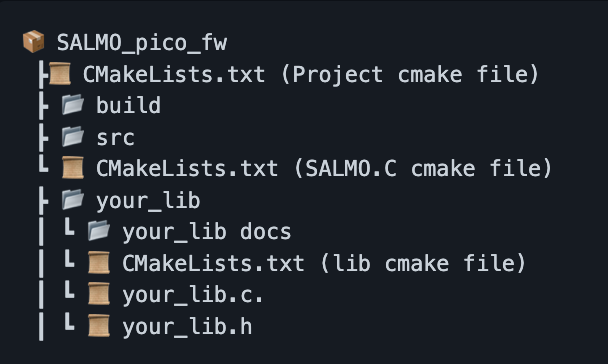
\includegraphics[scale=1]{figures/image73.png}
\captionsetup{type=figure}
\captionof{figure}{Struttura del codice di SALMO}
\end{center}

Ogni libreria contiene un proprio CMakeLists in cui viene specificato il
nome della libreria (linkando i file .c e .h) e linkando altre librerie
esterne (come \emph{pico\_stdlib}).

\begin{center}
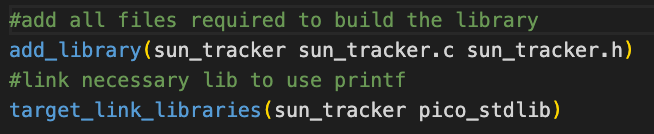
\includegraphics[scale=1]{figures/image45.png}
\captionsetup{type=figure}
\captionof{figure}{CMakeLists della libreria per il calcolo della posizione del sole}
\end{center}

Dopodichè nel main principale in cui verrà eseguito il codice (presente
in \emph{SALMO.c}), viene definito l'eseguibile (ovvero si linka il file
.c attribuendolo ad un nome), dopodiché si linkano le librerie definite
precedentemente per poi includere anche le cartelle in cui queste sono
presenti, per poi opzionalmente decidere se abilitare altri parametri
come \emph{usb output} o \emph{uart output.}

\begin{center}
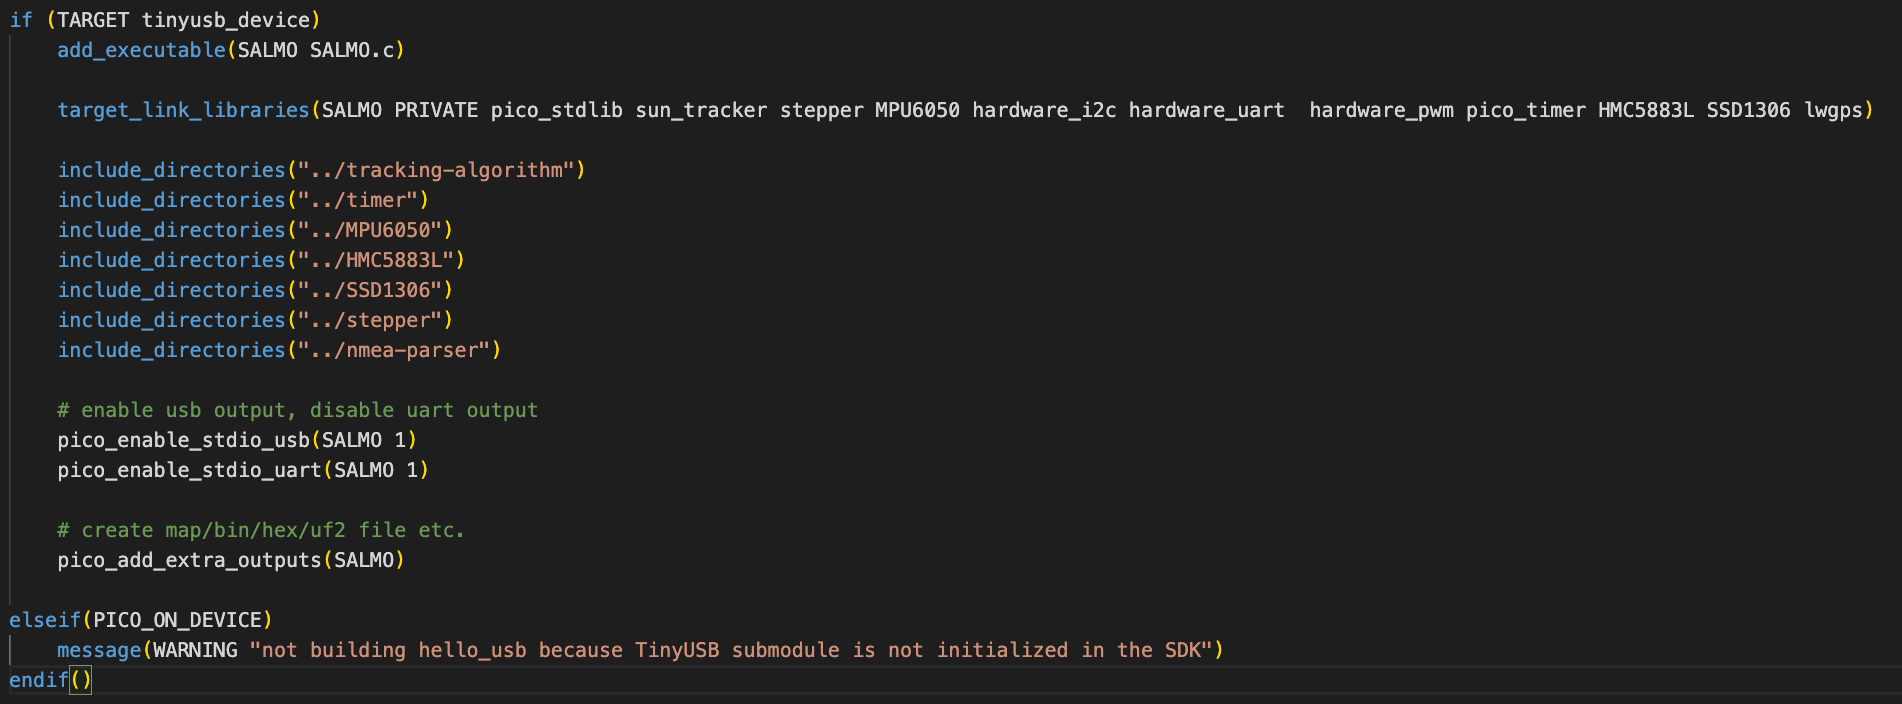
\includegraphics[scale=0.45]{figures/image66.png}
\captionsetup{type=figure}
\captionof{figure}{CMakeLists di SALMO.c}
\end{center}

I file CMakeLists vengono ``eseguiti'' in ordine gerarchico, per cui è
necessario avere un CMakeLists esterno che ha il compito di tenere
traccia di tutti gli altri \emph{CMakeLists} e di definire i parametri
relativi alla versione del \emph{CMAKE} e della versione del compilatore
C e C++. Per compilare il progetto SALMO è sufficiente quindi eseguire
il comando CMake sul file CMakeLists più esterno, producendo così un
Makefile che, una volta eseguito, compilerà autonomamente l'intero
progetto restituendo i file eseguibili necessari per flashare il
microcontrollore.

\begin{center}
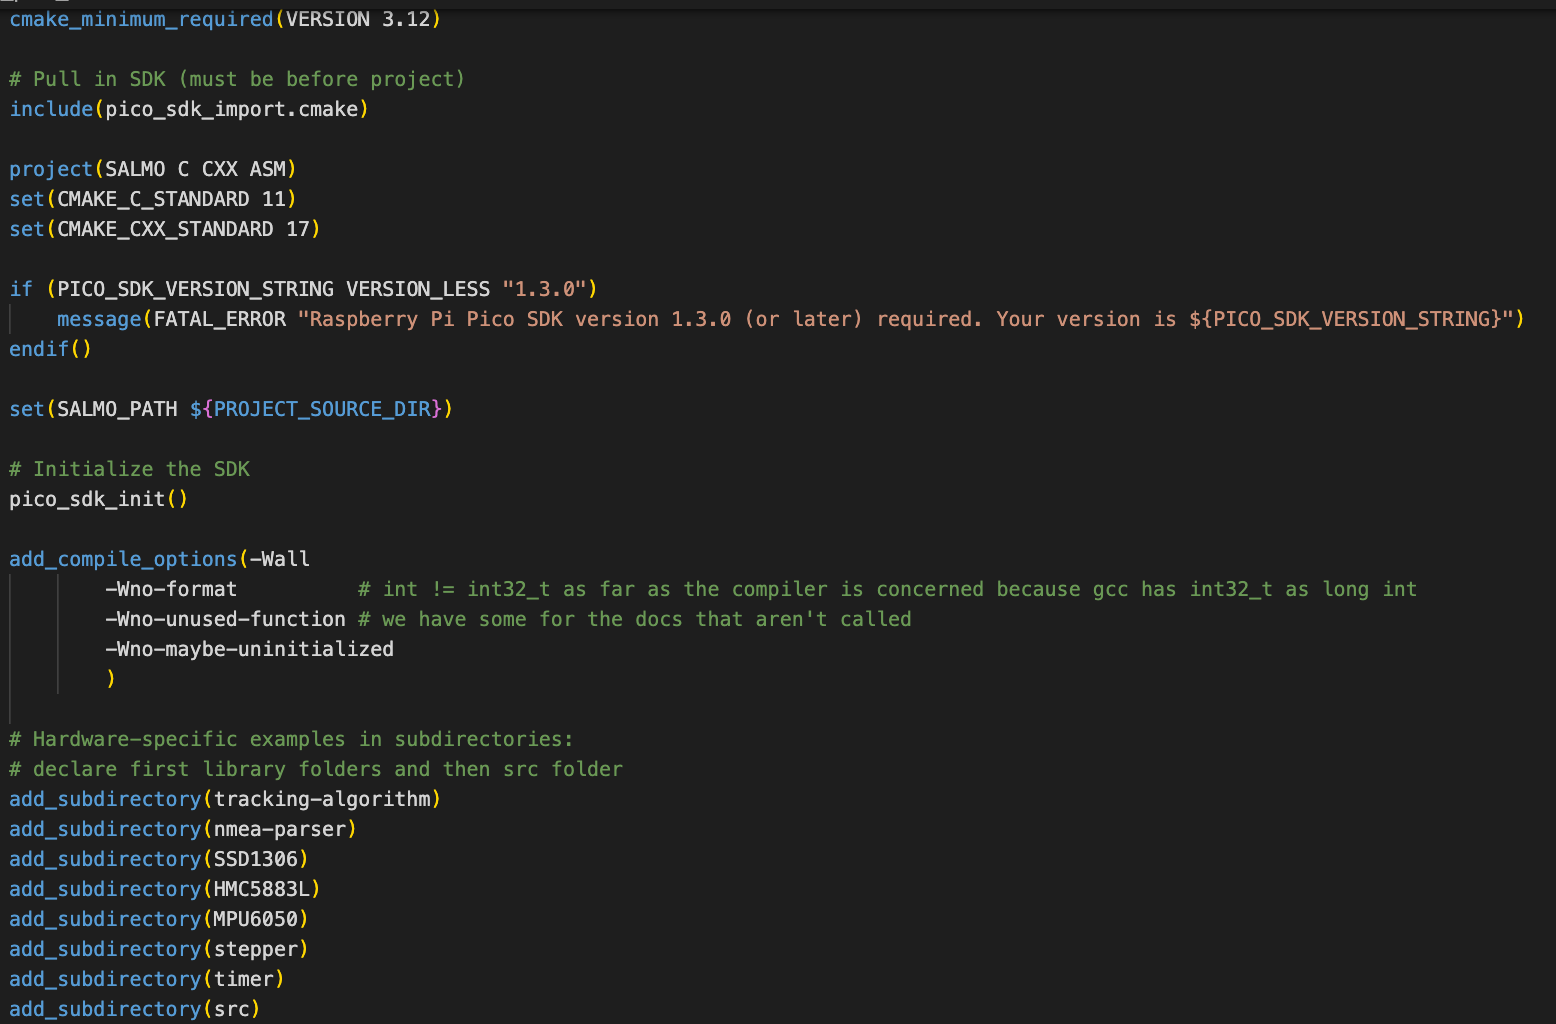
\includegraphics[scale=0.6]{figures/image67.png}
\captionsetup{type=figure}
\captionof{figure}{CMakeLists del progetto}
\end{center}

Per rendere più veloce la fase di compilazione abbiamo deciso di
scrivere tre piccoli script \emph{bash}, situati nella cartella
\emph{src}: \emph{build.sh}, \emph{flash.sh},
\emph{build\_and\_flash.sh}: lo script di build utilizza \emph{cmake}
per compilare i \emph{Makefile} e salvare i relativi eseguibili dentro
la cartella \emph{build}, mentre quello di flash utilizza
\emph{picotool} per caricare l'eseguibile in formato \emph{.uf2}
direttamente nella \emph{flash} del microcontrollore, anche se il RP2040
non si trova in bootloader mode (\emph{picotool} riavvia il MCU in
bootloader mode). Infatti se non usassimo \emph{picotool} dovremmo
resettare la scheda tenendo premuto il pulsante di boot per entrare in
bootloader mode, successivamente trascinare il file eseguibile
all'interno della partizione Mass Storage del micro, per poi resettarlo
via pulsante. Lo script di \emph{build} è inoltre dotato di un
\emph{flag} opzionale attivabile scrivendo \emph{./build.sh all}, con il
quale viene rimossa l'intera directory di build ed il progetto viene
ricompilato da capo (utile in caso di errori del compilatore non
realmente presenti nel codice). Abbiamo scelto di flashare mediante
l'eseguibile con estensione \emph{.uf2} in quanto, utilizzando questo
tipo di file, è sufficiente copiare l'eseguibile nella partizione di
tipo Mass Storage che il RP2040 offre una volta avviato in bootloader
mode.\\
Come intuibile, il file \emph{build\_and\_flash.sh} esegue sia le
operazioni di compilazione sia l'operazione di flashing.

\hypertarget{algoritmo-per-ottenere-la-posizione-del-sole}{%
\section{Algoritmo per ottenere la posizione del
sole}\label{algoritmo-per-ottenere-la-posizione-del-sole}}

Al fine di poter pilotare correttamente i motori verso il sole abbiamo
dovuto trovare un modo per convertire i dati ottenuti dal GPS in
elevazione ed azimuth del sole (espressi in gradi). Per approcciare
correttamente il problema abbiamo iniziato a leggere vari \emph{papers}
e relazioni tecniche riguardo ad algoritmi per la rilevazione della
posizione del sole, il primo, forse tra i più datati, è stato \emph{The
astronomical almanac's algorithm for approximate solar position} di
\emph{Joseph J. Michalsky}. Dopo alcune letture abbiamo capito che era
necessario passare tra vari sistemi di riferimento per ottenere le
coordinate del sole, in particolare ci siamo imbattuti nel concetto di
\emph{Julian Date} (giorni passati dalle 12 del 1 Gennaio 4713 B.C.),
coordinate celesti, \emph{GMST} (Greenwich Mean Sidereal Time, un giorno
siderale è 4 minuti più corto di un giorno solare) e \emph{LMST} (Local
Mean Sidereal Time). Nonostante nel paper di \emph{Michalsky} fosse
presente del codice \emph{FORTRAN} per l'implementazione dell'algoritmo,
non lo abbiamo ritenuto abbastanza ``solido'' ed efficiente per il
nostro tipo di applicazione.

Per poter verificare la corretta posizione del sole abbiamo utilizzato
questo sito come contro prova dei nostri calcoli:
\href{https://gml.noaa.gov/grad/solcalc/}{\underline{https://gml.noaa.gov/grad/solcalc/}}.

\begin{center}
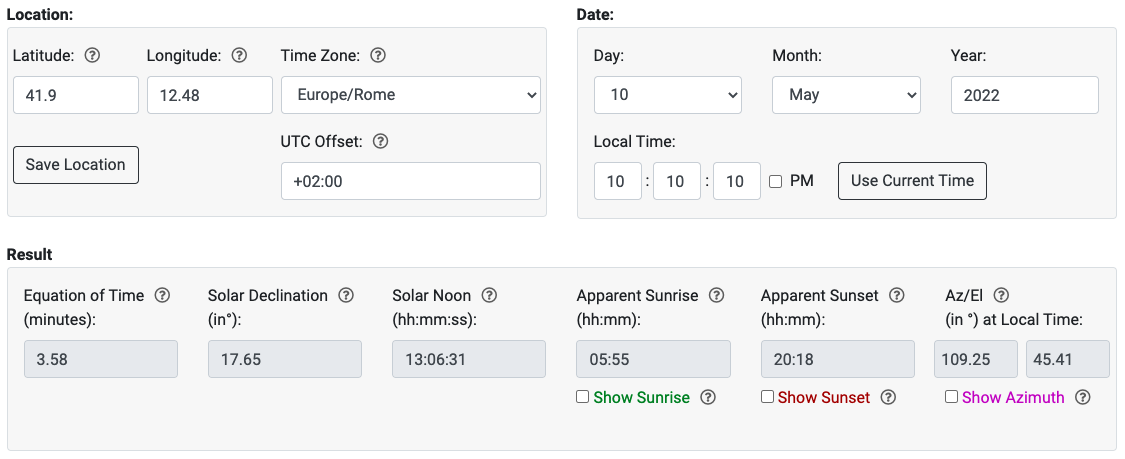
\includegraphics[scale=0.4]{figures/image72.png}
\captionsetup{type=figure}
\captionof{figure}{Interfaccia web NOAA solcalc}
\end{center}

Fortunatamente la \emph{NOAA} (National Oceanic and Atmospheric
Administration) oltre a fornire questa interfaccia web, condivide anche
i file \emph{excel} con cui vengono eseguiti i calcoli al fine di
ottenere gli stessi risultati presenti sul loro sito. Di conseguenza,
essendo questo \emph{tool} uno dei pochi affidabili in rete con cui
poter verificare i nostri calcoli, abbiamo deciso di riportare le
formule del file \emph{excel} in codice C per ottenere gli stessi
risultati. I calcoli intermedi non verranno riportati nel dettaglio in
quanto sono computazioni astronomiche che non rientrano nelle tematiche
trattate nel corso.

Per la computazione abbiamo fatto riferimento a due strutture dati, una
denominata \emph{Place} in cui viene salvata la data, l'orario e
latitudine e longitudine ``\emph{parsate}'' dal GPS (mediante una
libreria open source), e l'altra, \emph{Position,} in cui vengono
salvati tutti i parametri intermedi ed i risultati finali per il calcolo
della posizione del sole (basato sull'algoritmo della \emph{NOAA}).

\begin{center}
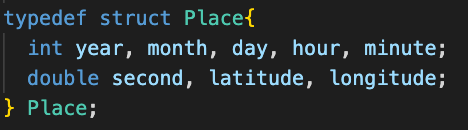
\includegraphics[scale=1]{figures/image25.png}
\captionsetup{type=figure}
\captionof{figure}{Struct "Place"}
\end{center}

\begin{center}
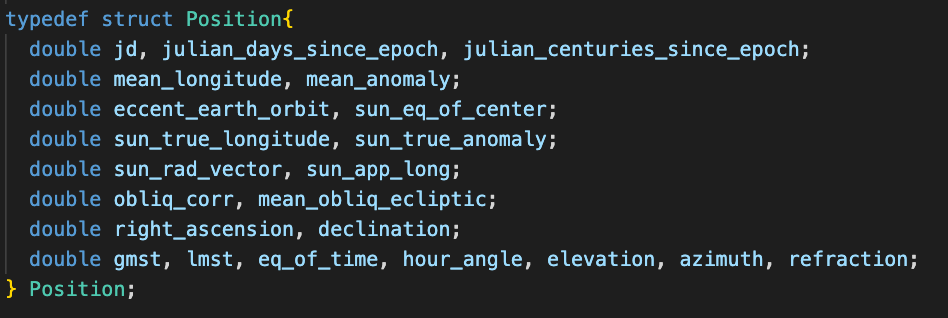
\includegraphics[scale=0.8]{figures/image33.png}
\captionsetup{type=figure}
\captionof{figure}{Struct "Position"}
\end{center}

Per calcolare la posizione esatta del sole infatti i dati contenuti in
\emph{Place} ven gono utilizzati per ottenere una \emph{Julian Date},
una \emph{Julian Date} conteggiata a partire dalle 12 del primo Gennaio
2000 e successivamente tutti i parametri intermedi per poi ottenere
elevazione e azimuth del sole. In seguito ad alcuni test abbiamo
riscontrato che siamo in grado di ottenere un'ottima precisione,
addirittura nell'ordine del grado!

\hypertarget{implementazione-software-delle-periferiche}{%
\section{Implementazione software delle
periferiche}\label{implementazione-software-delle-periferiche}}

Tutte le periferiche, a meno di GPS, utilizzano interfaccia di
comunicazione \emph{I2C}.

Il protocollo hardware \emph{I2C} prevede due linee seriali di
comunicazione: \emph{SDA} (Serial DAta) per i dati e \emph{SCL} (Serial
CLock) per il clock (la comunicazione I2C è di tipo sincrono).\\
Siccome le linee \emph{SDA} ed \emph{SCL} sono di tipo Open-Drain (o
Open-Collector a seconda della tecnologia utilizzata) sono necessari dei
resistori di pull-up per portare a livello logico alto le linee. Nel
progetto \emph{SALMO}, siccome accelerometro e magnetometro vengono
acquistati sotto forma di moduli commerciali, troviamo già i resistori
di pull-up su di essi, per cui, questi ultimi, verranno dimensionati e
montati direttamente in solo uno dei moduli (verranno quindi rimossi
dagli altri).

\begin{center}
\includegraphics[scale=0.2]{figures/image61.png}
\captionsetup{type=figure}
\captionof{figure}{Esempio di bus I2C}
\end{center}

La struttura dei driver di HMC5883L e MPU6050 segue una logica ben
precisa, in modo da rendere particolarmente semplice e versatile il
codice:

\begin{itemize}
\item
  \begin{quote}
  \textless drivername\textgreater\_defines.h
  \end{quote}
\item
  \begin{quote}
  \textless drivername\textgreater\_I2C.h
  \end{quote}
\item
  \begin{quote}
  \textless drivername\textgreater\_I2C.c
  \end{quote}
\item
  \begin{quote}
  \textless drivername\textgreater.c
  \end{quote}
\item
  \begin{quote}
  \textless drivername\textgreater.h
  \end{quote}
\end{itemize}

Utilizzando questa struttura è possibile innanzitutto separare tutte le
definizioni di registri ed indirizzi in un file header separato
(\textless drivername\textgreater\_defines.h) ed in secondo luogo, forse
vantaggio principale, è possibile dichiarare e definire le funzioni di
lettura e scrittura nel bus I2C in due soli file
(\textless drivername\textgreater\_I2C.h e
\textless drivername\textgreater\_I2C.c) in modo che il vero e proprio
driver (\textless drivername\textgreater.h e
\textless drivername\textgreater.c) rimanga completamente indipendente
dalle funzioni I2C. Questo, è particolarmente vantaggioso perché le
funzioni I2C sono dipendenti dal HAL offerto dall'SDK (e quindi in certo
senso dall'architettura), per cui nel caso in cui volessimo
ri-utilizzare i driver per un'altra architettura (es. STM32) sarebbe
sufficiente modificare solamente le due funzioni di lettura e scrittura
su bus I2C nel file \textless drivername\textgreater\_I2C.c .\\
Il microcontrollore offre due controller I2C: I2C0 ed I2C1. Nel progetto
SALMO viene utilizzato solo uno dei due controller, che viene condiviso
da accelerometro, magnetometro e display.\\
Tutte e 3 le periferiche utilizzano il bus in modalità fast, ovvero a
400KHz.\\
Per effettuare una lettura o la scrittura di un registro di una
periferica nel bus è necessario che il master invii un messaggio
specifico determinato dal protocollo I2C: bit di start, 7, 8 oppure 10
bit di indirizzo (HMC5883L utilizza 8 bit, mentre MPU6050 e SSD1306
utilizzano 7 bit di indirizzo), un bit che indica lettura o scrittura,
un bit di acknowledge da parte dello slave, e successivamente 8 bit di
dato (ad esempio il registro da leggere o il registro in cui si vuole
scrivere, seguito di nuovo da un bit di acknowledge. È possibile inviare
N blocchi da 8 bit seguiti dal bit di acknowledge dopo il bit di
read/write (anch'esso seguito da un bit di acknowledge).

\begin{center}
\includegraphics[scale=0.35]{figures/image51.png}
\captionsetup{type=figure}
\captionof{figure}{Data frame protocollo I2C}
\end{center}

Nel caso, ad esempio, in cui si voglia scrivere il contenuto di un
registro del MPU6050 è sufficiente inviare: bit di start, 7 bit di
indirizzo (LSB configurabile), bit di read (es. 0 1101000 1) che saranno
seguiti da un bit di acknowledge ed infine invieremo gli 8 bit
dell'indirizzo su cui vogliamo scrivere (es. 00111011). Successivamente
invieremo, dopo aver ricevuto l'acknowledge, i dati che vogliamo
scrivere.\\
Nel caso della lettura invece, è necessario ripetere la procedura
illustrata precedentemente fino all'invio dell'indirizzo del registro
(in questo caso da leggere) ed inviare però ora un bit di start seguito
dall'indirizzo dello slave ed infine un bit di read. La periferica slave
invierà finalmente, sempre dopo il bit di acknowledge, il contenuto del
registro richiesto.

\begin{center}
\includegraphics[scale=0.7]{figures/image39.png}
\captionsetup{type=figure}
\captionof{figure}{Data frame esempio lettura I2C}
\end{center}

\begin{center}
\includegraphics[scale=0.7]{figures/image35.png}
\captionsetup{type=figure}
\captionof{figure}{Funzioni di write e read I2C (driver MPU6050)}
\end{center}

Per quanto concerne l'implementazione software del display OLED, abbiamo
deciso di utilizzare la libreria già presente negli SDK di Raspberry
Pico (seppur per nulla completa). Sottolineiamo che attualmente il
driver di questa periferica non è stato completato poiché, non avendola
sotto mano, abbiamo deciso di prioritizzare il resto del lavoro.

Un altro protocollo di comunicazione utilizzato nel progetto è
\emph{UART} (\emph{Universal Asynchronous Receiver-Transmitter}), come
visto nel primo modulo del corso, permette il trasferimento e ricezione
di dati in seriale ad un tasso di velocità bit/s fissato, detto baud
rate. Abbiamo inserito la configurazione \emph{UART} nel modulo
\emph{PAM7Q.c}, file in cui vengono inizializzati i pin RX e TX, e
vengono settati tutti i parametri necessari a comporre il data frame,
assumendo la seguente configurazione:

\begin{itemize}
\item
  \begin{quote}
  Hardware flow: no
  \end{quote}
\item
  \begin{quote}
  Baud rate: 9600 bit/s
  \end{quote}
\item
  \begin{quote}
  Bit di dato: 8
  \end{quote}
\item
  \begin{quote}
  Bit di stop: 1
  \end{quote}
\item
  \begin{quote}
  Bit di parità: no
  \end{quote}
\end{itemize}

\begin{center}
\includegraphics[width=3.5in,height=1.5625in]{figures/image46.png}
\captionsetup{type=figure}
\captionof{figure}{Pacchetto gestito con comunicazione UART}
\end{center}

Il modulo GPS comunica in \emph{UART} con il microcontrollore mediante
protocollo a 9600 bit/s, codificando i messaggi con standard NMEA 1803
(National Marine Electronics Association). Per la lettura dei dati viene
popolato un buffer, di lunghezza 100 bytes, con ogni carattere ricevuto.
All'occorrenza del carattere \emph{``\textbackslash n''} la stringa
ricevuta viene salvata in un array di supporto, il buffer viene
successivamente svuotato e ricomincia la lettura per un numero pari a
\emph{GPS\_MAX\_SENTENCES}. Abbiamo inoltre deciso di comunicare con il
GPS in polling, anzichè utilizzare un interrupt, poiché interagendo con
il modulo ad intervalli ben definiti la seconda opzione avrebbe portato
ad un inutile overhead a causa della continua interruzione del
microcontrollore rispetto alle sue principali task.

Per tradurre le stringhe NMEA in informazioni utili alla struttura
\emph{Place}, definita nel modulo dell'algoritmo, è stata utilizzata una
libreria open source in grado di analizzare questi messaggi (vedasi
bibliografia). Tipicamente una stringa NMEA è composta nel seguente
modo:

\(\$ PREFISSO,dato1,dato2\ ...\ datoN - 1,datoN*CHECKSUM\)

In base al tipo di prefisso vengono trasferiti diversi tipi di dati, per
la nostra applicazione abbiamo fatto principale affidamento ai due
messaggi:

\begin{itemize}
\item
  \begin{quote}
  \$\emph{GPRMC}: fornisce la data (Anno, Mese, Giorno)
  \end{quote}
\item
  \begin{quote}
  \$\emph{GPGGA}: fornisce tempo (Ore, Minuti, Secondi), Latitudine,
  Longitudine.
  \end{quote}
\end{itemize}

Abbiamo valutato la correttezza del parsing utilizzando un tool online
(vedasi bibliografia)

\hypertarget{implementazione-driver-motori}{%
\section{Implementazione driver
motori}\label{implementazione-driver-motori}}

Il firmware di controllo dei motori è stato sviluppato partendo da una
libreria già esistente e open source disponibile su github ed è composta
da due file: \emph{pico\_stepper.h} e \emph{pico\_stepper.c}.

Nel primo è definita la \emph{struct} necessaria per inizializzare ogni
motore e gli \emph{header} delle funzioni implementate poi nel secondo
file.

Per interfacciarsi ai motori è stato necessario inizializzare la
\emph{struct} e i pin fisici delle 4 fasi, definire la velocità di
rotazione del motore, successivamente i motori vengono comandati
mediante la funzione \emph{step()}, che implementa il metodo ``wave
drive'', nel quale le fasi vengono pilotate in modo sequenziale da
un'onda quadra con un duty cycle del 25\%. La forma d'onda non è
generata tramite la periferica \emph{pwm} bensì in \emph{bit banging}
per semplicità di scrittura firmware dato che non erano necessarie
velocità elevate di commutazione.

\begin{center}
\includegraphics[scale=0.8]{figures/image50.png}
\captionof{figure}{Fasi per pilotaggio stepper unipolare}
\end{center}

\begin{center}
\includegraphics[scale=0.2]{figures/image44.png}
\captionsetup{type=figure}
\captionof{figure}{Output SALMO su oscilloscopio}
\end{center}

\hypertarget{funzionamento-generale-del-codice}{%
\section{Funzionamento generale del
codice}\label{funzionamento-generale-del-codice}}

\begin{center}
\includegraphics[scale=0.30]{figures/image36.png}
\captionsetup{type=figure}
\captionof{figure}{Flowchart del funzionamento del codice}
\end{center}

Come prima cosa vengono inizializzate le varie periferiche e moduli
ovvero:

\begin{itemize}
\item
  \begin{quote}
  UART
  \end{quote}
\item
  \begin{quote}
  USB CDC
  \end{quote}
\item
  \begin{quote}
  I2C
  \end{quote}
\item
  \begin{quote}
  Accelerometro
  \end{quote}
\item
  \begin{quote}
  Magnetometro
  \end{quote}
\item
  \begin{quote}
  Motore stepper
  \end{quote}
\end{itemize}

Dopodiché il microcontrollore entra in loop infinito in cui vengono
controllati degli input e delle variabili interne impostate dai timer.
Sono presenti tre timer che scandiscono:

\begin{itemize}
\item
  \begin{quote}
  Lettura input gps (ogni 4 secondi)
  \end{quote}
\item
  \begin{quote}
  Aggiornamento della posizione del motore (ogni 10 secondi)
  \end{quote}
\item
  \begin{quote}
  Aggiornamento posizione del sole mediante algoritmo (ogni 4 secondi)
  \end{quote}
\end{itemize}

Entrati nel loop infinito viene controllato, tramite interrupt, se il
pulsante di \emph{``Go home''} (\emph{SW3}) viene premuto, qualora
succeda, i motori vengono azionati per dirigere il pannello verso il
\emph{Nord} ottenuto dalla bussola ed a 45° di elevazione (tilt).
Successivamente viene verificato, sempre tramite interrupt, se il
pulsante di ``Tracking enable/disable'' (\emph{SW4}) viene premuto, in
questo caso il flag di tracking viene abilitato o disabilitato in base
al numero di iterazioni col pulsante, infatti ad ogni pressione il flag
viene negato, pertanto dopo averlo premuto una volta il motore rimarrà
in tracking mode e se il pulsante verrà azionato di nuovo il flag di
tracking verrà disabilitato. Alla scadenza del timer relativo al
tracking se il flag dovuto al pulsante è abilitato viene aggiornata la
posizione del motore. Dopodichè viene controllato se il timer relativo
alla lettura del gps è terminato, in caso affermativo viene eseguita la
lettura via uart ed il relativo parsing, infine viene controllato se il
timer relativo alla posizione del sole è scaduto, e di conseguenza viene
o meno eseguito il calcolo della posizione del sole basandosi sui dati
ottenuti dal GPS. Il programma poi ritorna nel loop principale e
continua il controllo delle variabili.

A causa della mancanza di accelerometro, pannello e struttura di
supporto per i motori, ulteriori \emph{feature} verranno implementate in
futuro.
\chapter{Assemblaggio della scheda}

L’assemblaggio della scheda è stato svolto in laboratorio sotto la supervisione
del Professore presso il laboratorio di elettronica del FabLab. 
In seguito all’arrivo delle PCB e dei componenti principali, abbiamo 
deposto la pasta saldante sulla scheda con l’aiuto dello stencil serigrafico
per procedere con la saldatura dei componenti con metodo \emph{thermal reflow}.\\
Al fine di tenere la scheda in posizione fissa, questa è stata inserita 
tra altre 4 schede fissate sul banco. Dopo aver passato la pasta saldante, 
abbiamo successivamente posizionato con particolare attenzione i componenti 
sulla scheda, controllando accuratamente il layout progettato in precedenza
ed aiutandoci con la BOM interattiva (che associa refdes e valore del componente
alla propria posizione sulla PCB).\\
Alcuni dei componenti realmente utilizzati
presentavano un modello diverso da quello previsto in fase di progettazione ma,
essendo una scheda di prototipazione e non una scheda di produzione, sono
risultati ugualmente adatti, senza alterare il funzionamento della scheda.
Infine, abbiamo fissato i componenti utilizzando una stazione di saldatura 
con piastra elettrica riscaldante, permettendo lo scioglimento delle sfere 
di stagno (contenute all’interno della pasta) e la conseguente saldatura 
dei dispositivi SMD.\\
Finito l’assemblaggio, ci siamo accorti che per una 
particolare scheda i pin del microcontrollore non sembravano essere fissati a
dovere ed infatti testando la sua alimentazione abbiamo potuto constatare il
surriscaldamento eccessivo del componente. Perciò per rimediare all’errore il
microcontrollore è stato dissaldato, ma nel farlo, le tre piste che collegavano
i rispettivi pin si sono alzate, non consentendo così l’utilizzo della scheda.\\
Un altro errore è sorto durante la fase di testing, infatti, misurando il 
segnale di comando in input ai motori, ci siamo accorti che al transistor a 
canale N montato sulla scheda era stata assegnata la piedinatura scorretta. 
Pertanto, abbiamo dovuto dissaldare i transistor atti al pilotaggio dei motori
per poi saldarli nuovamente nel verso corretto.


\begin{center}
\includegraphics[scale=0.4]{figures/image101.png}
\captionsetup{type=figure}
\captionof{figure}{Scheda SALMO completa di componenti essenziali}
\end{center}
\chapter{Testing della scheda}

Terminato l’assemblaggio, siamo passati alla fase di testing, in cui abbiamo verificato il funzionamento delle schede in tutti i loro aspetti.
Anzitutto abbiamo provato ad alimentarle via USB per verificare che la regolazione di tensione fosse funzionante. Abbiamo sfruttato il led sulla rail dei 3.3V come indicatore principale, poi abbiamo effettuato una misura più accurata tramite multimetro, appurando che il dimensionamento è stato fatto in modo corretto. Infatti sul testpoint della rail abbiamo misurato $3.3V \pm 0.05V$. \\
Dopo aver appurato che l’alimentazione fosse funzionante abbiamo flashato il microcontrollore con il codice che abbiamo sviluppato in parallelo su una dev-board Raspberry Pi Pico ed abbiamo verificato il corretto assemblaggio dei componenti. \\
Con un programma di prova abbiamo poi applicato un segnale di controllo ai motori e, analizzando l’uscita dello stadio con l’oscilloscopio, ci siamo accorti che in uscita non si aveva il segnale desiderato. Perciò prima abbiamo testato il segnale PWM generato dal microcontrollore, il quale è risultato corretto. Poi siamo passati al test sul MOSFET di pilotaggio. Qui ci siamo accorti che il segnale era sbagliato, quindi abbiamo intuito che il problema fossero i transistor. Il professore ci ha poi aiutati a capire nel dettaglio il problema misurando la tensione ai capi del diodo di protezione tra drain e source del MOSFET. Risultando un cortocircuito tra drain e source abbiamo capito che quelli non erano realmente il drain e il source del MOSFET e ci siamo accorti che, in fase di progetto, ai transistor a canale N montati sulla scheda era stata assegnata la piedinatura scorretta. Effettuando la misurazione di tensione tra i vari pin del transistor abbiamo capito quale fosse il gate ed abbiamo provveduto a dissaldare e risaldare i transistor nella posizione corretta. Dopo questa correzione il sistema di pilotaggio degli stepper è risultato funzionante.
I restanti componenti sono stati testati con diverse iterazioni del firmware e sono risultate perfettamente funzionanti. \\
Per concludere abbiamo misurato il consumo del prototipo all’avviamento dei motori e in modalità idle,  ricavando le seguenti misure:

\begin{itemize}
    \item consumo a motori attuati: $1-1.5 W$;
    \item consumo in idle: $0.2-0.4 W$;
\end{itemize}
I consumi dei motori sono risultati bassi grazie all’inerzia elevata dei riduttori.

\begin{center}
    \includegraphics[width=10cm]{figures/image3.png}
    \captionsetup{type=figure}
    \captionof{figure}{Consumi durante il movimento dei motori}
\end{center}

\begin{center}
    \includegraphics[width=10cm]{figures/image1.png}
    \captionsetup{type=figure}
    \captionof{figure}{Consumi durante lo stato di idle}
\end{center}

\begin{center}
    \includegraphics[width=15cm]{figures/image101.png}
    \captionsetup{type=figure}
    \captionof{figure}{La scheda in fase di testing}
\end{center}

\chapter{Implementazioni future}

Considerando i componenti mancanti, le funzionalità che vorremmo
implementare in un prossimo futuro sarebbero le seguenti:

\begin{itemize}
\item Interfaccia utente attraverso il display OLED
\item Sensing di tensione e corrente prodotti dal pannello
\item Struttura per pannello, motori e sensori
\item Interfaccia Python via COM port con visualizzazione valori, statistiche e controllo manuale motori
\end{itemize}

\noindent L'interfaccia utente nel display OLED mostrerà: tensione pannello e
corrente pannello, posizione del sole e posizione pannello (angolo di
Azimuth e angolo di Elevazione), orario e posizione geografica.

\begin{center}
\includegraphics[width=4.68229in,height=3.4426in]{figures/image27.png}
\captionsetup{type=figure}
\captionof{figure}{Esempio di interfaccia utente su display OLED}
\end{center}

\noindent La struttura di supporto per il pannello servirà prima di tutto a
consentire al pannello di muoversi nei due gradi di libertà (rotazione
intorno all'asse Z e rotazione intorno all'asse X) e poi per contenere
magnetometro ed accelerometro in modo che questi rilevino esattamente la
posizione del pannello (dovranno quindi essere fisicamente attaccati al
pannello e dovranno muoversi con esso).

\begin{center}
\includegraphics[width=3.63in,height=2.72in]{figures/image52.png}
\includegraphics[width=3.63in,height=2.72in]{figures/image68.png}
\includegraphics[width=3.63in,height=2.72in]{figures/image20.png}
\captionsetup{type=figure}
\captionof{figure}{Esempio di struttura di supporto per pannello e motori di tipo servo\\
(Credits:\href{https://www.thingiverse.com/thing:53321}{\underline{https://www.thingiverse.com/thing:53321}})}
\end{center}

\noindent Per quanto riguarda l'interfaccia grafica per la connessione seriale via
USB, si pensava di sviluppare in GUI (Graphical User Interface) in
linguaggio Python che consentisse di controllare manualmente le
posizioni dei motori, di abilitare il tracking o il return to home e
che, attraverso l'uso di piccoli grafici, mostrasse delle semplici
statistiche sulla potenza e l'energia prodotte dal pannello
fotovoltaico.

\begin{center}
\includegraphics[width=4.68229in,height=3.4426in]{figures/image47.png}
\captionsetup{type=figure}
\captionof{figure}{Esempio di GUI sviluppata in python}
\end{center}


\chapter{Conclusioni}

\hypertarget{resoconto-esperienza}{%
\section{\texorpdfstring{Resoconto esperienza
}{Resoconto esperienza }}\label{resoconto-esperienza}}

Il corso è stato formativo sotto tutti i punti di vista poiché abbiamo
potuto realizzare una scheda partendo da zero, cosa che negli altri
corsi non avevamo mai fatto. Per alcuni quindi è stata la prima PCB
progettata, perciò una tappa molto importante per il loro lavoro o
studio futuro. Inoltre il fatto di aver programmato il microcontrollore
con le poche basi di programmazione che avevamo dai corsi precedenti ci
ha permesso di imparare molto a livello firmware. Siccome il progetto
non è ancora completo, l'intenzione è quella di aggiungere man mano i
componenti mancanti al fine di avere la scheda più simile possibile a
quanto era stato programmato. Per concludere, i concetti imparati nel
modulo 1 del corso sono stati di fondamentale importanza per la
realizzazione della scheda, senza i quali sarebbe stato molto difficile
avere un'idea di come impostare il lavoro. L'obiettivo di progettare in
modo consono una scheda elettronica è dunque stato raggiunto.

\hypertarget{lezioni-imparate}{%
\section{Lezioni imparate}\label{Lezioni-imparate}}

\noindent Ragionando a posteriori su quanto abbiamo fatto, abbiamo stilato un
elenco di cosa avremmo potuto fare meglio e che cercheremo di applicare
nei progetti futuri:

\begin{itemize}
\item
  
  Il fanout del microcontrollore lo avremmo potuto fare esclusivamente
  con tracce da 0.2mm, senza ricorrere ad espansioni a 0.3mm, almeno per
  le tracce più corte. Questo avrebbe semplificato di non poco il
  routing di quella sezione;
  
\item
  
  Considerare fin da subito i return paths per i condensatori di
  decoupling. Nella realizzazione non abbiamo pensato a collegare alcuna
  traccia per il GND, perché ci siamo affidati ai poligoni di
  riempimento. Questo si è rivelato un problema, perché alla fine del
  progetto abbiamo riscontrato che molti riempimenti risultavano
  scollegati da GND e, soprattutto, che i percorsi effettivi delle linee
  di GND dei condensatori di bypass del microcontrollore sono risultati
  molto lunghi, il che rende quasi inutile il fatto di posizionarli
  vicini ai pin;
  
\item
  
  Controllare meglio il posizionamento dei refdes sul layer di
  silkscreen. Abbiamo realizzato solo a scheda prodotta che il refdes di
  C10 è stato posizionato sopra C14, rendendolo invisibile;
  
\item
  
  Controllare meglio i componenti scelti. Abbiamo infatti scelto di
  utilizzare un led rgb di un formato che in realtà si fatica a trovare sul
  mercato. Anche questo è stato scoperto solo in fase di assemblaggio.
  
\end{itemize}
\chapter{Bibliografia}

\begin{itemize}
\item
  \begin{quote}
  \href{https://github.com/raspberrypi/pico-sdk}{\underline{Repository
  Pico SDK}}
  \end{quote}
\item
  \begin{quote}
  \href{https://github.com/raspberrypi/pico-examples}{\underline{Repository
  Pico Examples}}
  \end{quote}
\item
  \begin{quote}
  \href{https://github.com/raspberrypi/picotool}{\underline{Repository}
  \underline{Picotool}}
  \end{quote}
\item
  \begin{quote}
  \href{https://raspberrypi.github.io/pico-sdk-doxygen/}{\underline{Documentazione
  Pico SDK}}
  \end{quote}
\item
  \begin{quote}
  \href{https://datasheets.raspberrypi.com/pico/raspberry-pi-pico-c-sdk.pdf}{\underline{Raspberry
  Pi Pico C/C++ SDK}}
  \end{quote}
\item
  \begin{quote}
  \href{https://datasheets.raspberrypi.com/rp2040/hardware-design-with-rp2040.pdf}{\underline{Hardware
  design with RP2040}}
  \end{quote}
\item
  \begin{quote}
  \href{https://www.researchgate.net/publication/222131147_The_Astronomical_Almanac's_algorithm_for_approximate_solar_position_1950-2050}{\underline{The
  astronomical almanac's algorithm for approximate solar position}}
  \end{quote}
\item
  \begin{quote}
  \href{https://www.nrel.gov/docs/fy08osti/34302.pdf}{\underline{Solar
  Position Algorithm for Solar Radiation Applications}}
  \end{quote}
\item
  \begin{quote}
  \href{https://github.com/jrowberg/i2cdevlib/blob/master/STM32/HMC5883/HMC5883L.h}{\underline{Repository
  driver HMC5883L STM32}}
  \end{quote}
\item
  \begin{quote}
  \href{https://github.com/Harinadha/STM32_MPU6050lib/blob/master/MPU6050.h}{\underline{Repository
  driver MPU6050 STM32}}
  \end{quote}
\item
  \begin{quote}
  \href{https://github.com/kosma/minmea}{\underline{Repository NMEA
  parser minmea}}
  \end{quote}
\item
  \begin{quote}
  \href{https://github.com/beshrkayali/pico_stepper}{\underline{Repository
  pico stepper driver}}
  \end{quote}
\item
  \begin{quote}
  \href{https://swairlearn.bluecover.pt/nmea_analyser}{\underline{Tool
  online per analisi stringhe NMEA}}
  \end{quote}
\item
  \begin{quote}
  \href{https://www.thingiverse.com/thing:53321}{\underline{Thingiverse
  dual axis solar tracker}}
  \end{quote}
\end{itemize}

\chapter{Allegati}

\hypertarget{gerbers}{%
\section{Gerbers}\label{gerbers}}
Si allegano i seguenti documenti, in scala 1:1, nell'ordine specificato:


\begin{enumerate}
    \item B\_Cu
    \item B\_Mask
    \item B\_Silkscren
    \item Edge\_Cuts
    \item F\_Cu
    \item F\_Mask
    \item F\_Paste 
    \item F\_Silkscreen
    \item Drill map (non in scala)
\end{enumerate}

\includepdf[pages={1}]{figures/gerbers/PPSE_2021-B_Cu.pdf}
\includepdf[pages={1}]{figures/gerbers/PPSE_2021-B_Mask.pdf}
\includepdf[pages={1}]{figures/gerbers/PPSE_2021-B_Silkscreen.pdf}
\includepdf[pages={1}]{figures/gerbers/PPSE_2021-Edge_Cuts.pdf}
\includepdf[pages={1}]{figures/gerbers/PPSE_2021-F_Cu.pdf}
\includepdf[pages={1}]{figures/gerbers/PPSE_2021-F_Mask.pdf}
\includepdf[pages={1}]{figures/gerbers/PPSE_2021-F_Paste.pdf}
\includepdf[pages={1}]{figures/gerbers/PPSE_2021-F_Silkscreen.pdf}
\includepdf[pages={1}]{figures/gerbers/PPSE_2021-drl_map.pdf}

\section{BOM}\label{gerber}
Si allega di seguito la distinta base con tutti i componenti presenti sulla scheda
\includepdf[pages={1-}]{figures/BOM_PPSE.pdf}

\end{document}
